%//==============================--@--==============================//%
\documentclass{kons-5}
\usepackage{extra-math-utils}
\usepackage{customtitlepage}
\usepackage{customboxes}
\usepackage{duckuments}

%------------------------------TITLE PAGE-----------------------------%
\title{%
    Apontamentos PROE \\ 
    \large (Alguns tópicos \href{https://github.com/Kons-5}{\large \faGithub})
}
\department{Engenharia Eletrotécnica e de Computadores}
\exam{Propagação e Radiação de Ondas Eletromagnéticas}

\universitylogo{img/title-page/IST.pdf}
\titleimage{img/title-page/Magnetic-discussion}
%\titleimagecaption{Sistema Multiple Input Multiple Output (MIMO)}

%% Add Authors here
\addauthor{João Gonçalves}{99995}{jrazevedogoncalves@tecnico.ulisboa.pt}
\addauthor{Teresa Nogueira}{100029}{maria.teresa.ramos.nogueira@tecnico.ulisboa.pt}

\date{Novembro 2023}
%---------------------------------------------------------------------%

\renewcommand{\epsilon}{\varepsilon}
% \captionsetup{belowskip=-1.25em}

\begin{document}
    %% title page
    \maketitle

    % preface
    %//==============================--@--==============================//%
\section*{Guia para a Leitura deste Resumo}

Este resumo foi elaborado para facilitar o estudo e a compreensão dos conceitos fundamentais em \href{https://fenix.tecnico.ulisboa.pt/disciplinas/PROE/2023-2024/1-semestre}{\textit{Propagação e Radiação de Ondas Eletromagnéticas}}. Para aproveitar ao máximo este material, recomenda-se:
\begin{itemize}
    \item \textbf{Leitura Sequencial:} Embora cada secção (ou quase todas) seja auto-contida, uma leitura sequencial ajudará a construir uma compreensão progressiva dos conceitos, desde os mais básicos até aos mais complexos.

    \item \textbf{Uso de Recursos Complementares:} Recomenda-se a consulta de livros, artigos e outros materiais adicionais sugeridos nas notas. Estes oferecem perspetivas diferentes e aprofundadas sobre os tópicos abordados.

    \item \textbf{Complemento às Aulas:} É importante ressaltar que este resumo serve como um complemento às aulas e não como um substituto. As aulas proporcionam uma experiência de aprendizagem com oportunidades para discussão e de esclarecimento de dúvidas.

\end{itemize}

Em termos de notação, tudo o que tiver mais do que uma dimensão será representado a negrito (i.e., vetores, matrizes, $\dots$). Vetores unitários (ou versores) são representados a negrito e têm um chapeu em cima (e.g., $\mathbf{\hat{u}}$).

Contribuições e relatos de quaisquer inconsistências ou erros encontrados são bem-vindos através de \textit{issues} no \href{https://github.com/kons-5/IST-PROE-Notes}{{\large \faGithub}}.

%//==============================--@--==============================//%
\section*{Resultados da Análise de Fourier}

\subsection*{Série de Fourier}

A série de Fourier de uma função periódica $\mathrm{f}(t)$ com período $T$ é uma expansão em termos de funções seno e cosseno que são ortogonais no intervalo \([0, T]\), e é dada por:
$$
    \mathrm{f}(t) \equiv \frac{a_0}{2} + \sum_{n=1}^{\infty} \left[ a_n \cos\left(\frac{2\pi n t}{T}\right) + b_n \sin\left(\frac{2\pi n t}{T}\right) \right]
$$
onde os coeficientes $a_0$, $a_n$ e $b_n$ são calculados como:
$$
    a_0 = \frac{2}{T} \int_{0}^{T} \mathrm{f}(t) \, dt 
    \quad \text{(valor médio/componente DC)}
$$
$$
    a_n = \frac{2}{T} \int_{0}^{T} \mathrm{f}(t) \cos\left(\frac{2\pi n t}{T}\right) \, dt,
    \qquad
    b_n = \frac{2}{T} \int_{0}^{T} \mathrm{f}(t) \sin\left(\frac{2\pi n t}{T}\right) \, dt
$$
Estes coeficientes representam a amplitude das frequências no espectro de $\mathrm{f}(t)$.

\subsection*{Transformada de Fourier}

A transformada de Fourier é uma ferramenta matemática fundamental que permite a análise de funções no domínio da frequência.
$$
    \begin{aligned}
        \mathrm{F}(\omega) \equiv \mathcal{F}\{ f(t) \}
        &\overset{\underset{\mathrm{def}}{}}{=}
        \int_{-\infty}^{\infty} f(t)\, e^{-j\omega t} \, dt
        & &\text{(equação de análise)}
        \\
        \mathrm{f}(t) \equiv \mathcal{F}^{-1}\{ F(\omega ) \}
        &\overset{\underset{\mathrm{def}}{}}{=}
        \int_{-\infty}^{\infty} F(\omega)\, e^{j\omega t} \, \frac{d\omega}{2\pi}
        & &\text{(equação de síntese)}
    \end{aligned}
$$

%//==============================--@--==============================//%
\section*{Algumas Identidades do Cálculo Vetorial}

$$
    \begin{aligned}
        &\nabla \times (\nabla \phi) = 0 
        & &\qquad \text{Rotacional do gradiente de um campo escalar é zero.}
        \\
        &\nabla \cdot (\phi \nabla \psi) = \phi \nabla^2 \psi + \nabla \phi \cdot \nabla \psi
        & &\qquad \text{Divergência do produto escalar por gradiente.}
        \\
        &\nabla \cdot (\phi \nabla \psi - \psi \nabla \phi) = \phi \nabla^2 \psi - \psi \nabla^2 \phi
        & &\qquad \text{Divergência do produto de gradientes escalares.}
        \\
        &\nabla \cdot (\phi \mathbf{A}) = (\nabla \phi) \cdot \mathbf{A} + \phi \nabla \cdot \mathbf{A}
        & &\qquad \text{Divergência do produto de um escalar por um vetor.}
        \\
        &\nabla \times (\phi \mathbf{A}) = (\nabla \phi) \times \mathbf{A} + \phi \nabla \times \mathbf{A}
        & &\qquad \text{Rotacional do produto de um escalar por um vetor.}
        \\
        &\nabla \cdot (\nabla \times \mathbf{A}) = 0
        & &\qquad \text{Divergência do rotacional de um vetor é zero.}
        \\
        &\nabla \cdot (\mathbf{A} \times \mathbf{B}) = \mathbf{B} \cdot (\nabla \times \mathbf{A}) - \mathbf{A} \cdot (\nabla \times \mathbf{B})
        & &\qquad \text{Divergência do produto vetorial.}
        \\
        &\nabla \times (\nabla \times \mathbf{A}) = \nabla (\nabla \cdot \mathbf{A}) - \nabla^2 \mathbf{A}
        & &\qquad \text{Rotacional do rotacional de um vetor.}
    \end{aligned}
$$
%//==============================--@--==============================//%

    %% table of contents
    \customtoc
    
    %% body
    \pagestyle{custom}
    
    \chapter{Conceitos Fundamentais}{img/1/Chapter-1-img}
        %//==============================--@--==============================//%
\section{Equações de Maxwell}
\label{sec:maxwell-eq}

É necessário um conjunto de quatro vetores para descrever os fenómenos do campo eletromagnético:
\begin{itemize}
    \item[] o campo elétrico, $\mathbf{E}$ (unidades: V/m, volt por metro)
    \item[] o campo de indução magnética, $\mathbf{B}$ (unidades: T, tesla)
    \item[] o campo de deslocamento elétrico, $\mathbf{D}$ (unidades: C/m$^2$, coulomb por metro quadrado)
    \item[] o campo magnético, $\mathbf{H}$ (unidades: A/m, ampère por metro)
\end{itemize}

Para fenómenos eletromagnéticos variáveis no tempo consideraram-se as equações de Maxwell:
$$
    \left\{
    \begin{aligned}%
        \nabla \times \mathbf{E} &= -\dfrac{\partial \mathbf{B}}{\partial t} 
        & &\qquad\text{\small (Lei de Indução)} \\
        \nabla \cdot \mathbf{D} &= \rho_{ext} 
        & &\qquad\text{\small (Lei de Gauss)} \\
        \nabla \times \mathbf{H} &= \mathbf{J}_{ext} + \dfrac{\partial \mathbf{D}}{\partial t} 
        & &\qquad\text{\small (Lei de Ampère com a correção de Maxwell)} \\
        \nabla \cdot \mathbf{B} &= 0 
        & &\qquad\text{\small (Lei de Gauss para o magnetismo)}
    \end{aligned}
    \right.
$$
As quantidades $\rho_{ext}$ $[$C/m$^3]$ e $\mathbf{J}_{ext}$ $[$A/m$^2]$ representam a densidade de carga volumétrica e a densidade de corrente elétrica (fluxo de carga) de quaisquer cargas externas (ou seja, excluindo quaisquer cargas e correntes de polarização induzidas no meio).

As densidades de carga e corrente, $\rho_{ext}$ e $\mathbf{J}_{ext}$, podem ser consideradas como as fontes dos campos eletromagnéticos. Em problemas de propagação de ondas, estas densidades estão localizadas no espaço; por exemplo, estão restritas a fluir numa antena. Os campos elétricos e magnéticos gerados são irradiados a partir destas fontes e podem propagar-se para grandes distâncias até às antenas recetoras.

Longe de geradores (\textit{sources}), i.e., em regiões do espaço livres de fontes (\textit{source-free regions}), as equações de Maxwell tomam uma forma mais simples, em que se considera que $\rho_{ext} = 0$ e $\mathbf{J}_{ext} = 0$.


O mecanismo qualitativo pelo qual as equações de Maxwell originam campos eletromagnéticos que se propagam pode ser visualizado com o seguinte exemplo:

\begin{figure}[H]
    \centering
    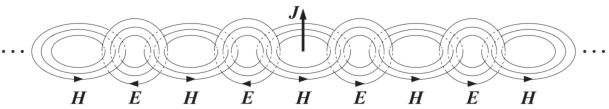
\includegraphics[width=0.7\linewidth]{img/1/Propagacao-de-ondas.pdf}
    \caption{Propagação do campo eletromagnético~\cite{orfanidis2008electromagnetic}}
\end{figure}

\begin{check}
    Uma corrente $\mathbf{J}$ que varia no tempo numa antena linear gera um campo magnético $\mathbf{H}$ circulante e também variável no tempo. Este campo magnético, através da lei de Faraday, origina um campo elétrico $\mathbf{E}$ circulante, que, segundo a lei de Ampère, gera um campo magnético, e assim por diante. Os campos elétricos e magnéticos interligados propagam-se para longe da fonte de corrente.
\end{check}

%//==============================--@--==============================//%
\subsection{Conservação de Carga}

Maxwell adicionou o termo da corrente de deslocamento à lei de Ampère para garantir a conservação da carga. De facto, ao tomarmos a divergência de ambos os lados da lei de Ampère e usando a lei de Gauss $\nabla \cdot \mathbf{D} = \rho$, obtemos:
$$ 
    \nabla \cdot (\nabla \times \mathbf{H}) = \nabla \cdot \mathbf{J}_{ext} + \frac{\partial}{\partial t}(\nabla \cdot \mathbf{D}) = \nabla \cdot \mathbf{J}_{ext} + \frac{\partial \rho_{ext}}{\partial t} 
$$
Usando a identidade vetorial $\nabla \cdot (\nabla \times \mathbf{H}) = 0$, obtemos a forma diferencial da lei de conservação da carga:
$$ 
    \boxed{\frac{\partial \rho_{ext}}{\partial t} + \nabla \cdot \mathbf{J}_{ext} = 0} \quad \text{(conservação da carga)} 
$$

%//==============================--@--==============================//%
\section{Relações Constitutivas e Meios Materiais}

As densidades de fluxo elétrico e magnético, $\mathbf{D}$ e $\mathbf{B}$, estão relacionadas com as intensidades de campo $\mathbf{E}$ e $\mathbf{H}$ através das chamadas \textit{relações constitutivas}, cuja forma precisa depende do material no qual os campos existem. No vácuo, assumem a sua forma mais simples:
$$
    \boxed{%
        \begin{aligned}
            \mathbf{D} &= \epsilon_{0} \mathbf{E} \\
            \mathbf{B} &= \mu_{0} \mathbf{H}
        \end{aligned}
    }
    \quad\rightarrow\quad
    \left\{
    \begin{aligned}
        \epsilon_{0} &\approx 8.854 \cdot 10^{-12} \; [\text{F/m}]\\
        \mu_{0} &\approx 4\pi \cdot 10^{-7} \; [\text{H/m}]
    \end{aligned}\right.
$$
onde $\epsilon_{0}$ e $\mu_{0}$ são a permitividade e permeabilidade do vácuo, respetivamente.

A partir de $\epsilon_{0}$ e $\mu_{0}$, podemos definir outras duas constantes, nomeadamente, a velocidade da luz e a impedância característica do vácuo:
$$
    \boxed{%
        c_0 = \frac{1}{\sqrt{\epsilon_{0} \mu_{0}}} = 3 \cdot 10^8 \; [\text{m/s}], 
        \quad
        \eta_0 = \sqrt{\frac{\mu_{0}}{\epsilon_{0}}} \approx 120\pi\; [\Omega]
    }
$$

A forma mais simples das relações constitutivas é para dielétricos simples, homogéneos e isotrópicos, e para materiais magnéticos:
$$
    \boxed{%
    \begin{aligned}
        \mathbf{D} &= \epsilon \mathbf{E} \\
        \mathbf{B} &= \mu \mathbf{H}
    \end{aligned}
    }
$$
Esta relação é tipicamente válida para frequências mais baixas. A permitividade $\epsilon$ e a permeabilidade $\mu$ estão relacionadas com as suscetibilidades elétrica e magnética dos materiais, i.e.,
$$
    \boxed{%
    \begin{aligned}
        \epsilon &= \epsilon_{0} (1 + \chi)  \\
        \mu &= \mu_{0} (1 + \chi_m)
    \end{aligned}
    }
$$
As suscetibilidades $\chi$ e $\chi_m$ são medidas das propriedades de polarização elétrica e magnética do material. Por exemplo, temos para a densidade do fluxo elétrico:
$$
    \mathbf{D} = \epsilon \mathbf{E} = \epsilon_{0} (1 + \chi) \mathbf{E} = \epsilon_{0} \mathbf{E} + \epsilon_{0} \chi \mathbf{E} = \epsilon_{0} \mathbf{E} + \mathbf{P}
$$
onde $\mathbf{P} = \epsilon_{0} \chi \mathbf{E}$ representa a polarização dielétrica do material, isto é, o momento dipolar elétrico médio por unidade de volume. Num material magnético, temos:
$$
    \mathbf{B} = \mu_0 (\mathbf{H} + \mathbf{M}) = \mu_0 (\mathbf{H} + \chi_m \mathbf{H}) = \mu_0 (1 + \chi_m) \mathbf{H} = \mu \mathbf{H}
$$
onde $\mathbf{M} = \chi_m \mathbf{H}$ é a magnetização, isto é, o momento magnético médio por unidade de volume. A velocidade da luz no material e a impedância característica são:
$$
    c = \frac{1}{\sqrt{\mu \epsilon}} , \quad \eta = \sqrt{\frac{\mu}{\epsilon}}
$$
A permitividade e a permeabilidade relativa, e o índice de refração de um material são definidos por:
$$
    \epsilon_{r} = \frac{\epsilon}{\epsilon_{0}} = 1 + \chi, \quad \mu_{r} = \frac{\mu}{\mu_0} = 1 + \chi_m, \quad n = \sqrt{\epsilon_{r} \mu_{r}}
$$
Podemos relacionar a velocidade da luz e a impedância do material com os correspondentes valores no vácuo:
$$
c = \frac{1}{\sqrt{\mu \epsilon}} = \frac{1}{\sqrt{\mu_0 \epsilon_{0} \epsilon_{r} \mu_{r}}} = \frac{c_0}{\sqrt{\epsilon_{r} \mu_{r}}} = \frac{c_0}{n}
$$
$$
    \eta = \sqrt{\frac{\mu}{\epsilon}} = \sqrt{\frac{\mu_0 \mu_{r}}{\epsilon_{0} \epsilon_{r}}} = \eta_0 \sqrt{\frac{\mu_{r}}{\epsilon_{r}}} = \eta_0 \frac{\mu_r}{n} = \eta_0 \frac{n}{\epsilon_r}
$$
Para um material não magnético, temos $\mu = \mu_0$ ou $\mu_r = 1$, e a impedância simplifica para $\eta = \eta_0/n$.

%//==============================--@--==============================//%

De uma forma mais geral, as relações constitutivas podem ser não homogéneas, anisotrópicas, não lineares, dependentes da frequência (dispersivas) ou todas as anteriores. 

Em \textit{materiais não homogéneos}, a permitividade depende da localização dentro do material:
$$
    \mathbf{D}(\mathbf{r},t) = \epsilon(\mathbf{r}) \mathbf{E}(\mathbf{r},t)
$$

Em \textit{materiais anisotrópicos}, $\epsilon$ depende das direções $x$, $y$, $z$ e as relações constitutivas podem ser escritas em forma de matriz (ou tensor):
$$
    \begin{bmatrix}
        D_x \\
        D_y \\
        D_z \\
    \end{bmatrix} =
    \begin{bmatrix}
        \epsilon_{xx} & \epsilon_{xy} & \epsilon_{xz} \\
        \epsilon_{yx} & \epsilon_{yy} & \epsilon_{yz} \\
        \epsilon_{zx} & \epsilon_{zy} & \epsilon_{zz} \\
    \end{bmatrix}
    \begin{bmatrix}
        E_x \\
        E_y \\
        E_z \\
    \end{bmatrix}
$$
A anisotropia é uma propriedade inerente da estrutura atómica/molecular do dielétrico. Também pode ser causada pela aplicação de campos externos.

Em \textit{materiais não lineares}, $\epsilon$ pode depender da magnitude  $E$ do campo elétrico aplicado na forma:
$$
    \mathbf{D} = \epsilon (E) \mathbf{E}, \quad \text{onde} \quad \epsilon(E) = \epsilon + \epsilon_2 E^2 + \epsilon_3 E^3 + \ldots
$$
Uma consequência típica da não linearidade é causar harmónicas de ordem superior.

Materiais com uma constante dielétrica dependente da frequência, $\epsilon(\omega)$, são referidos como \textit{dispersivos}. A dependência da frequência surge porque quando um campo elétrico variável no tempo é aplicado, a resposta de polarização do material \underline{não pode ser instantânea}. Tal resposta dinâmica pode ser descrita pela relação constitutiva convolucional (e causal):
$$
    \mathbf{D}(\mathbf{r}, t) = \int_{-\infty}^{t} \epsilon(t - t') \mathbf{E}(\mathbf{r}, t') dt'
$$
que se torna multiplicativa no domínio da frequência:
$$
    \underline{\mathbf{D}}(\mathbf{r}, \omega) = \epsilon(\omega) \underline{\mathbf{E}}(\mathbf{r}, \omega)
$$
Na realidade, todos os materiais são dispersivos. Contudo, $\epsilon(\omega)$ tipicamente exibe uma forte dependência de $\omega$ apenas para certas frequências. 


%//==============================--@--==============================//%
\subsection{Eletrodinâmica Macroscópica}

As densidades $\rho_{ext}$ e $\mathbf{J}_{ext}$ representam as cargas e correntes externas ou livres num meio material. A polarização induzida $\mathbf{P}$ e a magnetização $\mathbf{M}$ podem ser tornadas explícitas nas equações de Maxwell através das relações constitutivas:
$$
    \mathbf{D} = \epsilon_0 \mathbf{E} + \mathbf{P}, \quad \mathbf{B} = \mu_0 (\mathbf{H} + \mathbf{M})
$$
Assim, podemos escrever as equações de Maxwell em termos dos campos $\mathbf{E}$ e $\mathbf{B}$:
$$
    \begin{aligned}
        \nabla \times \mathbf{E} &= -\frac{\partial \mathbf{B}}{\partial t}
        &
        \nabla \times \mathbf{B} &= \mu_0 \epsilon_0 \frac{\partial \mathbf{E}}{\partial t} + \mu_0 \mathbf{J}_{ext} + \mu_0 \frac{\partial \mathbf{P}}{\partial t} + \mu_0 \nabla \times \mathbf{M}
        \\
        \nabla \cdot \mathbf{E} &= \frac{1}{\epsilon_0} (\rho - \nabla \cdot \mathbf{P})
        &
        \nabla \cdot \mathbf{B} &= 0
    \end{aligned}
$$
Identificamos assim as densidades de corrente e carga devido à polarização do material como: 
$$
    \mathbf{J}_{pol} = \frac{\partial \mathbf{P}}{\partial t}, \quad \rho_{pol} = -\nabla \cdot \mathbf{P}
$$
Da mesma forma, a quantidade $\mathbf{J}_{mag} = \nabla \times \mathbf{M}$ pode ser identificada como a corrente de magnetização. 

Para um meio dielétrico e condutor (e.g., plasma), acresce-se à lei de Ampère a componente $\mathbf{J}_{cond} = \sigma \mathbf{E}$. As densidades totais de corrente e carga, num meio material genérico, são:

$$
    \mathbf{J}_{tot} 
    = 
    \eqnmarkbox[blue]{free1}{\mathbf{J}_{ext}} + \eqnmarkbox[red]{bound1}{\mathbf{J}_{cond} + \mathbf{J}_{pol} + \mathbf{J}_{mag}}
    = 
    \eqnmarkbox[blue]{free2}{\mathbf{J}_{ext}} + \eqnmarkbox[red]{bound2}{\sigma \mathbf{E} + \frac{\partial \mathbf{P}}{\partial t} + \nabla \times \mathbf{M}}
$$
\annotatetwo{above, label below}{free1}{free2}{macro currents}
\annotatetwo{below, label above}{bound1}{bound2}{micro currents}

\vspace*{-0.75em}
$$
    \rho_{tot} = \rho + \rho_{pol} = \rho - \nabla \cdot \mathbf{P}
$$
e podem ser considerados como as fontes dos campos.

\begin{check}
    Estas relações satisfazem as equações de Maxwell macroscópicas,
    $$
        \boxed{%
            \nabla \times \mathbf{E} = -\frac{\partial \mathbf{B}}{\partial t},
            \quad
            \nabla \times \mathbf{H} = \mathbf{J}_{ext} + \sigma \mathbf{E} + \dfrac{\partial \mathbf{D}}{\partial t}
        }
    $$
    A resposta material (dipolar) está "oculta" nos vetores de polarização e magnetização $\mathbf{P}$ e $\mathbf{M}$, respetivamente.
\end{check}

%//==============================--@--==============================//%
\subsection{Modelos Simples de Dielétricos e Condutores}

Um modelo simples para as propriedades dielétricas de um material pode ser obtido considerando o movimento de um eletrão ligado na presença de um campo elétrico aplicado. À medida que o campo elétrico tenta separar o eletrão do núcleo positivamente carregado, cria-se um momento de dipolo elétrico. A média deste momento de dipolo ao longo do volume do material dá origem a um momento de dipolo macroscópico por unidade de volume.

Um modelo simples para a dinâmica do deslocamento $\mathbf{r}$ do eletrão ligado é o seguinte (onde $\dot{\mathbf{r}} = d\mathbf{r}/dt$):
$$
    m\ddot{\mathbf{r}} = e \mathbf{E} - k\mathbf{r} - m\Gamma\dot{\mathbf{r}}
    \quad \text{(modelo Drude-Lorentz)}
$$
onde assumimos que o campo elétrico está a atuar na direção $\mathbf{r}$ e que existe uma força restauradora tipo-mola devido à ligação do eletrão ao núcleo, e uma força de atrito proporcional à velocidade do eletrão.

A constante da mola $k$ está relacionada à frequência de ressonância da mola pela relação $\omega_0 = \sqrt{k/m}$, ou $k = m\omega_0^2$. Assim, podemos reescrever a equação como:
$$
    \boxed{%
        \ddot{\mathbf{r}} + \Gamma\dot{\mathbf{r}} + \omega_0^2 \mathbf{r} = \frac{e}{m} \mathbf{E}
    }
$$
O termo friccional $\Gamma\dot{\mathbf{r}}$ surge de colisões que tendem a desacelerar o eletrão. O parâmetro $\Gamma$ é uma medida da taxa de colisões por unidade de tempo, e, portanto, $\tau = 1/\Gamma$ representará o tempo médio entre colisões.

\begin{check}
    A ideia básica deste modelo é que o campo elétrico aplicado tende a separar cargas positivas de cargas negativas, criando assim um momento de dipolo elétrico. Neste sentido, o modelo contém as características básicas de outros tipos de polarização em materiais.
\end{check}


%//==============================--@--==============================//%
\subsubsection{Meio Dielétrico Dispersivo}

O campo elétrico aplicado pode ter qualquer dependência temporal. Em particular, se assumirmos que é sinusoidal com frequência $\omega$, então, a equação modelo terá a solução $\mathbf{r} = \Re\{\mathbf{\underline{r}} e^{j\omega t}\}$, onde o fasor $\mathbf{\underline{r}}$ deve satisfazer:
$$
    -\omega^2 \mathbf{\underline{r}} + j\omega \Gamma \mathbf{\underline{r}} + \omega_0^2 \mathbf{\underline{r}} = \frac{e}{m} \mathbf{\underline{E}}
    \implies
    \mathbf{\underline{r}} = \frac{e/m}{\omega_0^2 - \omega^2 + j\omega\Gamma}\, \mathbf{\underline{E}}
$$
Podemos encontrar assim a polarização por unidade de volume no domínio da frequência, $\mathbf{\underline{P}}$. Supondo que existem $N$ dipolos elementares por unidade de volume e admitindo o momento de dipolo elétrico individual $\mathbf{\underline{p}} = e\mathbf{\underline{r}}$, vem:
$$
    \mathbf{\underline{P}} = N \mathbf{\underline{p}} = Ne\mathbf{\underline{r}} = \frac{Ne^2}{m} \frac{1}{\omega_0^2 - \omega^2 + j\omega\Gamma}\, \mathbf{\underline{E}} \equiv \epsilon_0 \chi(\omega) \mathbf{\underline{E}}
$$
A densidade do fluxo elétrico será: $\mathbf{\underline{D}} = \epsilon_0 \mathbf{\underline{E}} + \mathbf{\underline{P}} = \epsilon_0 (1 + \chi(\omega)) \mathbf{\underline{E}} = \epsilon(\omega) \mathbf{\underline{E}}$, onde a permitividade efetiva $\epsilon(\omega)$ é:
$$
    \boxed{%
        \epsilon(\omega) = \epsilon_0 \left( 1 + \frac{\omega_p^2}{\omega_0^2 - \omega^2 + j\omega\Gamma} \right)
    }
    \quad \text{onde} \quad
    \omega_p = \sqrt{\frac{N e^2}{\epsilon_0 m}} \quad \text{(frequência de plasma)}
$$
este modelo para $\epsilon(\omega)$ é conhecido como um ``dielétrico de Lorentz''.

\begin{warning}
    As partes real e imaginária de $\epsilon(\omega)$ caracterizam as propriedades \emph{refrativas} e \emph{absorventes} do material. Por convenção, definimos a parte imaginária com o sinal negativo (porque usamos a dependência temporal $e^{j\omega t}$):
    $$
        \epsilon(\omega) = \epsilon'(\omega) - j\epsilon''(\omega), \quad \text{onde}
    $$
    $$
            \epsilon'(\omega) = \Re\{\epsilon(\omega)\} = \epsilon_0 + \frac{\epsilon_0\omega_p^2(\omega_0^2 - \omega^2)}{(\omega_0^2 - \omega^2)^2 + \Gamma^2\omega^2} 
            \qquad\qquad
            \epsilon''(\omega) = -\Im\{\epsilon(\omega)\} = \frac{\epsilon_0\omega_p^2\Gamma\omega}{(\omega_0^2 - \omega^2)^2 + \Gamma^2\omega^2}
    $$
    \vspace{-1.5em}
    \begin{figure}[H]
        \centering
        \begin{subfigure}[b]{0.45\linewidth}
            \centering
            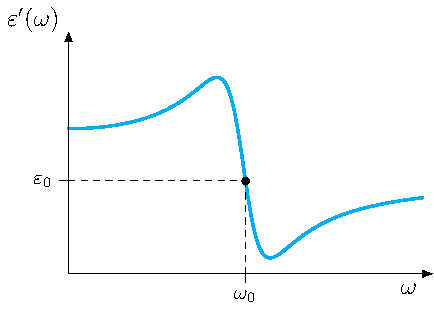
\includegraphics[width=\linewidth]{img/1/Epsilon_real.pdf}
        \end{subfigure}\hfil
        \begin{subfigure}[b]{0.45\linewidth}
            \centering
            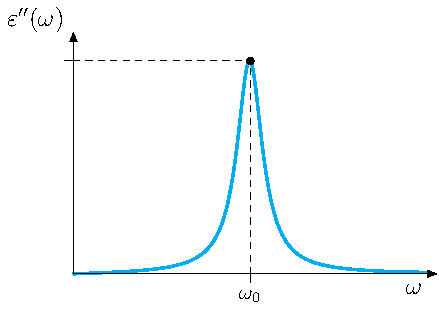
\includegraphics[width=\linewidth]{img/1/Epsilon_imag.pdf}
        \end{subfigure}
        \caption{Partes real e imaginária da permitividade efetiva $\epsilon(\omega)$.}
    \end{figure}

    \footnotetext{A componente $\epsilon'$ representa a permitividade sem perdas, i.e., $\epsilon' = \epsilon_0 \epsilon_r$. $\epsilon''$ é a componente imaginária da permitividade atribuída às cargas ligadas e relaxamento dipolar, que originam perdas de energia indistinguíveis das perdas devido à condução de cargas.}
\end{warning}

%//==============================--@--==============================//%
\subsubsection{Meio Condutor Dispersivo}

As propriedades de condutividade de um material são descritas pela lei de Ohm. Para derivar esta lei do nosso modelo simples, usamos a relação $\mathbf{J} = \rho \dot{\mathbf{r}}$, onde a densidade de carga de condução é $\rho = Ne$. Consequentemente,
$$
    \mathbf{\underline{J}} = \rho (j\omega\mathbf{\underline{r}}) = \frac{j\omega Ne^2}{m} \frac{1}{\omega_0^2 - \omega^2 + j\omega\Gamma}\, \mathbf{\underline{E}} \equiv \sigma(\omega)\mathbf{\underline{E}}
$$
e, portanto, identificamos a condutividade $\sigma(\omega)$:
$$
    \sigma(\omega) = \frac{j\omega Ne^2}{m} \frac{1}{\omega_0^2 - \omega^2 + j\omega\Gamma} = \frac{j\omega\epsilon_0\omega_p^2}{\omega_0^2 - \omega^2 + j\omega\Gamma}
    \overset{\substack{\text{para}\\\text{$\omega_0 = 0$}\vspace{1mm}}}{\:\implies}
    \sigma(\omega) = \frac{\epsilon_0 \omega^{2}_{p}}{\Gamma + j\omega}
    \quad \text{``modelo de Drude''}
$$
Notamos que $\sigma(\omega)/j\omega$ é essencialmente a suscetibilidade elétrica considerada anteriormente. De facto, temos $\mathbf{\underline{J}} = j\omega \mathbf{\underline{P}}$, e portanto, $\mathbf{\underline{P}} = \mathbf{\underline{J}}/j\omega = (\sigma(\omega)/j\omega) \mathbf{\underline{E}}$. Segue-se que $\epsilon(\omega) - \epsilon_0 = \sigma(\omega)/j\omega$, e
$$
    \epsilon(\omega) = \epsilon_0 + \frac{\epsilon_0\omega_p^2}{\omega_0^2 - \omega^2 + j\omega\Gamma} = \epsilon_0 + \frac{\sigma(\omega)}{j\omega}
$$

%//==============================--@--==============================//%
\subsection{Material Genérico} \label{sec:material-generico-dispersivo}

Para descrever um material com ambas as \underline{propriedades dielétricas e condutivas}, podemos tomar a suscetibilidade como a soma de dois termos, um que descreve as cargas polarizadas ligadas e o outro as cargas de condução livres. Assumindo parâmetros diferentes $\{ \omega_0, \omega_p, \Gamma \}$ para cada termo, obtemos a permitividade total:
$$
    \epsilon(\omega) 
    =
    \epsilon_0 \Big[ 1 + \chi_d(\omega) + \chi_c(\omega) \Big]
    =
    \epsilon_0 
    + 
    \frac{\epsilon_0 \omega_{dp}^2}{\omega_{d0}^2 - \omega^2 + j\omega \Gamma_d} 
    + 
    \frac{\epsilon_0 \omega_{cp}^2}{\omega_{c0}^2 - \omega^2 + j\omega \Gamma_c}
$$
Agrupando os dois primeiros termos em $\epsilon_d(\omega)$ e denotanto o terceiro por $\sigma_c(\omega)/j\omega$, obtemos a permitividade efetiva total do material:
$$
    \boxed{%
        \epsilon(\omega) = \epsilon_d(\omega) + \frac{\sigma_c(\omega)}{j\omega}
    }
    \quad \text{(permitividade efetiva total)}
$$

\begin{check}
    Semelhante a $\mathbf{\underline{D}}$ e $\mathbf{\underline{E}}$, a indução e o campo magnético estão ligados por uma permeabilidade magnética complexa $\mu(\omega)$ tal que $\mathbf{\underline{B}} = \mu(\omega)\mathbf{\underline{H}}$. Substituindo $\mathbf{\underline{D}} = \epsilon(\omega)\mathbf{\underline{E}}$ e $\mathbf{\underline{B}} = \mu(\omega)\mathbf{\underline{H}}$ nas equações macroscópicas de Maxwell, descobre-se que:
    $$
        \nabla \times \mathbf{\underline{E}} = -j\omega\mu(\omega)\mathbf{\underline{H}},
        \quad
        \nabla \times \mathbf{\underline{H}} = \mathbf{\underline{J}}_{ext} + j\omega\epsilon(\omega)\mathbf{\underline{E}}, 
    $$
    onde $\epsilon (\omega)$ é a permitividade complexa equivalente acima, que inclui as contribuições das correntes de condução e das correntes de polarização.
\end{check}

Admitindo $\epsilon_d(\omega) = \epsilon'_d(\omega) - j\epsilon''_d(\omega)$, como visto anteriormente, e assumindo que a condutividade $\sigma_c(\omega)$ é real para a gama de frequências de interesse, podemos definir $\epsilon(\omega) = \epsilon'(\omega) - j\epsilon''(\omega)$, onde:
$$
    \epsilon'(\omega) = \epsilon'_d(\omega), \qquad \epsilon''(\omega) = \epsilon''_d(\omega) + \frac{\sigma_c(\omega)}{\omega}
$$
Uma maneira conveniente de quantificar as perdas é através da tangente de perdas (\textit{loss tangent}) definida em termos das partes real e imaginária da permitividade efetiva:
$$
    \boxed{ \tan \theta = \frac{\epsilon''(\omega)}{\epsilon'(\omega)} } \quad \text{onde $\theta$ é o ângulo de perdas.}
$$
%//==============================--@--==============================//%
        %//==============================--@--==============================//%
\section{Ondas Planas}
\label{sec:ondas-planas}

%//==============================--@--==============================//%
\subsection{Equações de Onda livres de Fontes}
\label{sec:eq-onda-sem-fonte}

Para meios isotrópicos padrão (sem dispersão), numa região isenta de fontes onde  $\rho = 0$ e $\mathbf{J}_{ext} = 0$, as equações de Maxwell podem ser reescritas da seguinte forma:
\begin{align}
    \nabla\times \mathbf{E} &= -\mu\,\frac{\partial \mathbf{H}}{\partial t} & \nabla\times \mathbf{H} &= \epsilon\,\frac{\partial \mathbf{E}}{\partial t}\label{eq:1} \\
    \nabla\cdot \mathbf{E} &= 0 & \nabla\cdot \mathbf{H} &= 0\label{eq:2}
\end{align}

As equações diferenciais de primeira ordem podem ser unificadas numa única equação diferencial de segunda ordem, em $\mathbf{E}$ ou em $\mathbf{H}$. Aplicando o rotacional a (\ref{eq:1}) obtemos:
\begin{equation}
        \nabla \times (\nabla \times \mathbf{E}) = -\mu\,\dfrac{\partial}{\partial t}\left(\nabla \times \mathbf{H}\right)
\end{equation}
Por conseguinte, substituindo com a equação par em (\ref{eq:1}), obtemos:
\begin{equation}
    \nabla\times (\nabla \times \mathbf{E}) = -\mu\epsilon\,\frac{\partial^2 \mathbf{E}}{\partial t^2}
\end{equation}
Com recurso à identidade vetorial e admitindo a equação (\ref{eq:2}), é possivel reescrever:
\begin{equation}
     \nabla \times (\nabla \times \mathbf{E}) = \nabla(\nabla\cdot\mathbf{E}) - \nabla^2\mathbf{E} = - \nabla^2\mathbf{E}
\end{equation}
Finalmente obtemos:
\begin{equation} \label{eq:wave-eq}
    \boxed{\nabla^2\mathbf{E} -\mu\epsilon\,\frac{\partial^2 \mathbf{E}}{\partial t^2} = 0}
    \quad\text{e de forma análoga}\quad
    \boxed{\nabla^2\mathbf{H} -\mu\epsilon\,\frac{\partial^2 \mathbf{H}}{\partial t^2} = 0}
\end{equation}

\vspace{-0.75em}
\begin{warning}
    A equação de onda é de segunda ordem, nas coordenadas temporais e espaciais. Utilizamos $\nabla^2$ para representar o operador \emph{Laplaciano}; podemos, portanto, escrever as equações de \eqref{eq:wave-eq} em cada coordenada do campo.
\end{warning}

Uma equação de onda \underline{unidimensional} genérica tem a forma e solução como se apresenta:
$$
    \frac{\partial^2 \mathbf{u}}{\partial x^2} - \frac{1}{c^2} \frac{\partial^2 \mathbf{u}}{\partial t^2} = 0
    \;\implies\;
    \boxed{%
        \mathbf{u} = f(x - ct) + g(x + ct)
    }
    \quad \text{(variação espacial em apenas uma das direções)}
$$

%//==============================--@--==============================//%
\subsection{Regime Harmónico no Tempo}

Dado que as equações de Maxwell são equações diferenciais lineares, variações temporais sinusoidais impostas pelo gerador de funções com uma frequência específica produzirão variações sinusoidais de $\mathbf{E}$ e $\mathbf{H}$ com a mesma frequência no estado estacionário.

O campo elétrico $\mathbf{E}(\mathbf{r}, t) $ em regime harmónico pode ser reescrito em termos da amplitude complexa na forma de fasor $\underline{\mathbf{E}}(\mathbf{r})$ na forma:
\begin{equation}
    \mathbf{E}(\mathbf{r}, t) = \Re\left\{\underline{\mathbf{E}}(\mathbf{r}) e^{j\omega t}\right\}
\end{equation}
As amplitudes complexas dos campos satisfazem as equações de Maxwell independentes do tempo:
\begin{equation}
    \nabla\times\underline{\mathbf{E}} = -j\omega\underline{\mathbf{B}}\qquad
     \nabla\times\underline{\mathbf{H}} = \underline{\mathbf{J}}_{ext} + j\omega\underline{\mathbf{D}}
\end{equation}
e por conseguinte
\begin{equation}\label{eq:time-independent-max}
    \boxed{\nabla\times\underline{\mathbf{E}} = -j\omega\mu\underline{\mathbf{H}}\qquad
     \nabla\times\underline{\mathbf{H}} = \underline{\mathbf{J}}_{ext} + j\epsilon\omega\underline{\mathbf{E}}}
\end{equation}

%//==============================--@--==============================//%
\subsection{Propriedade das Ondas Planas}
As ondas planas são a solução mais simples das equações de Maxwell. Por definição, um campo de onda plana é descrito por:
\begin{equation}
    \underline{\mathbf{E}} = \underline{\mathbf{E}}_0\, e^{-j \mathbf{k}\cdot\mathbf{r}}\qquad
    \underline{\mathbf{H}} = \underline{\mathbf{H}}_0\, e^{-j \mathbf{k}\cdot\mathbf{r}}
\end{equation}
O termo $e^{-j \mathbf{k}\cdot\mathbf{r}}$ é conhecido como fator de propagação, pois determina a variação espacial dos campos. É expresso em termos das coordenadas do ponto de observação $\mathbf{r} = (x, y, z)$ e em termos do vetor de onda fundamental $\mathbf{k} = (k_x, k_y, k_z)$.

É conveniente escrever o fator de propagação em termos de um vetor unitário $\mathbf{\hat{d}}$ e um fator k denominado número de onda. Em meios isotrópicos, $\mathbf{\hat{d}}$ determina a direção de propagação da onda.
\begin{equation}
    \boxed{e^{-j \mathbf{k}\cdot\mathbf{r}} = e^{-j k\,\mathbf{\hat{d}}\cdot\mathbf{r}}}
\end{equation}
O comprimento de onda $\lambda$ é a distância pela qual a fase da onda sinusoidal muda por $2\pi$ radianos. Uma vez que o fator de propagação $e^{-j k\,\mathbf{\hat{d}}\cdot\mathbf{r}}$ acumula uma fase de $k$ radianos por metro, temos por definição que $k\lambda = 2\pi$. O comprimento de onda $\lambda$ pode ser expresso através da frequência da onda em hertz, $f = \omega/2\pi$, como se segue:
\begin{equation}
    \boxed{\lambda = \frac{2\pi}{k} = \frac{c}{f}}
\end{equation}

\begin{warning}
    Se o meio de propagação for o espaço livre, usamos os valores de vácuo dos parâmetros $\{\epsilon, \mu, c, \eta\}$, ou seja, $\{\epsilon_0, \mu_0, c_0, \eta_0\}$. O comprimento de onda no espaço livre e o número de onda correspondente são:
    \begin{equation}
        \lambda_0 = \frac{2\pi}{k_0} = \frac{c_0}{f} , \quad k_0 = \frac{\omega}{c_0}  
    \end{equation}
    Num dielétrico com índice de refração $n = \sqrt{\epsilon_r\mu_r}$, a velocidade da luz $c$, o comprimento de onda $\lambda$ e a impedância característica $\eta$ são todos reduzidos por um factor de $n$ em comparação com os valores no espaço livre, enquanto que o número de onda $k$ é aumentado por um factor de $n$:
    \begin{equation}
        c = \dfrac{c_0}{n}, \quad\eta = \dfrac{\eta_0}{n}, \quad\lambda = \dfrac{\lambda_0}{n}, \quad k = nk_0
    \end{equation}
\end{warning}

%//==============================--@--==============================//%
\clearpage
\subsection{Ondas Planas em Meios sem Perdas} \label{sec:ondas-sem-perdas}

Em materiais uniformes não dispersivos, com $\epsilon, \mu$ independentes de $\mathbf{r} = (x, y, z)$. As ondas planas satisfazem as equações de Maxwell sem fonte ($\mathbf{J} = 0$), definidas em (\ref{eq:time-independent-max}).

A variação no espaço de uma onda plana é controlada pelo fator de propagação $e^{-j \mathbf{k}\cdot\mathbf{r}}$. Assim:
\begin{equation}
    \begin{aligned}
        \nabla \times \mathbf{\underline{E}} &= \left( \frac{\partial}{\partial x}, \frac{\partial}{\partial y}, \frac{\partial}{\partial z} \right)  \times
         \left(\mathbf{\underline{E}}_0 e^{-j\mathbf{k}\cdot \mathbf{r}}\right) = \\[2pt]
         &=
         \left( \frac{\partial}{\partial x}, \frac{\partial}{\partial y}, \frac{\partial}{\partial z} \right)
         \times
         \left(\underline{E}_x,\underline{E}_y,\underline{E}_z\right) =
         \left(
             \frac{\partial \underline{E}_z}{\partial y} - \frac{\partial \underline{E}_y}{\partial z}, 
             \frac{\partial \underline{E}_x}{\partial z} - \frac{\partial \underline{E}_z}{\partial x},
             \frac{\partial \underline{E}_y}{\partial x} - \frac{\partial \underline{E}_x}{\partial y}
         \right)
    \end{aligned}
\end{equation}
Recorrendo ao cálculo das derivadas em todas as componente:
\begin{equation}
    -j\eqnmarkbox[blue]{curl}{\left(
     \underline{E}_{0z} k_y - \underline{E}_{0y} k_z,
     \underline{E}_{0x} k_z - \underline{E}_{0z} k_x,
     \underline{E}_{0y} k_x - \underline{E}_{0x} k_y
    \right)} \cdot e^{-j\mathbf{k}\cdot \mathbf{r}}
\end{equation}

\annotate{below, right}{curl}{$(k_x,k_y,k_z)\times(\underline{E}_{0x},\underline{E}_{0y},\underline{E}_{0z})$}
\noindent Consequentemente,
\begin{equation}
     \boxed{-j\mathbf{k}\times\underline{\mathbf{E}}_0\,e^{-j\mathbf{k}\cdot \mathbf{r}} = -j\mathbf{k}\times\mathbf{\underline{E}}}
\end{equation}
É então possível reescrever as equações de Maxwell:
\begin{equation}\label{eq:Max-k}
    \boxed{\mathbf{k}\times\mathbf{\underline{E}} =\omega\mu\mathbf{\underline{H}}\qquad
    \mathbf{k}\times\mathbf{\underline{H}} = -\omega\epsilon\mathbf{\underline{E}}}
\end{equation}
\begin{check}
    A equação à esquerda implica que $\mathbf{H}$ é perpendicular a ambos $\mathbf{k}$ e $\mathbf{E}$. Similarmente, a equação à direita mostra que $\mathbf{E}$ é perpendicular a ambos $\mathbf{k}$ e $\mathbf{H}$. Assim, os três vetores são mutuamente perpendiculares e dizemos que a onda é eletromagnética transversal (\textit{transverse electromagnetic}, TEM). Formalmente podemos escrever:

    \begin{equation}
        \mathbf{k}\cdot\mathbf{\underline{E}} = \mathbf{k}\cdot\mathbf{\underline{H}} = 0\qquad\mathbf{\underline{E}}\cdot\mathbf{\underline{H}} = 0
    \end{equation}
\end{check}
Os vetores $\mathbf{\underline{E}},\, \mathbf{\underline{H}},\, \mathbf{k}$ ou, analogamente\footnote{É conveniente escrever o vetor de onda em termos de um vetor unitário (ou versor) $\mathbf{\hat{d}}$ e um escalar $k$: $\mathbf{k} = k\mathbf{\hat{d}}.$ O escalar $k$ é o número de onda. Em meios isotrópicos padrão, o vetor $\mathbf{\hat{d}}$ determina a direção de propagação da onda.~\cite{silveirinha2023}}, $\mathbf{\underline{E}},\, \mathbf{\underline{H}},\, \mathbf{\hat{d}}$ formam uma base direita do espaço. As oscilações do campo são prependiculares à direção de propagação.

\vspace{-0.75em}
\begin{minipage}[c]{0.35\linewidth}
    \begin{figure}[H]
        \centering
        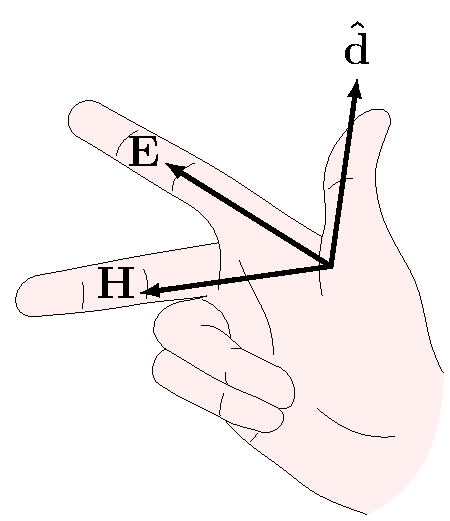
\includegraphics[width=0.75\linewidth]{img/1/Right-hand-basis.pdf}
        \caption{Base direita do espaço.}
    \end{figure}
\end{minipage}\hfill
\begin{minipage}[c]{0.65\linewidth}
    Substituindo $k = \omega\sqrt{\mu\epsilon} = n \cdot \omega/c $ em \eqref{eq:Max-k} e utilizando $k = \mathbf{k}\cdot\mathbf{\hat{d}}$, obtemos a seguinte relação explícita entre os campos e a direção de propagação da onda:
    \begin{equation}
        \boxed{ \mathbf{H} = -\frac{1}{\eta}\mathbf{\hat{d}} \times \mathbf{E}, \quad \mathbf{E} = \eta\mathbf{H} \times \mathbf{\hat{d}} }
    \end{equation}
    O produto vetorial roda efetivamente o campo relevante por 90°.
    \begin{warning}
        Esta relação é sempre válida para ondas planas em meios uniformes não dispersivos!
    \end{warning}
\end{minipage}

\vspace{0.5em}
A ligação entre a frequência angular e o número de onda implica que também existe uma ligação entre os períodos de tempo e espaço da onda. Podemos escrever:

\vspace{0.5em}
\begin{equation}
    \frac{\eqnmarkbox[blue]{T}{T}}{\lambda} = \frac{2\pi}{\omega} = \frac{2\pi}{k}\,\frac{n}{c} = \eqnmarkbox[red]{S}{\lambda}\, \frac{n}{c}
\end{equation}

\annotate{above, label below}{T}{período temporal}
\annotate{below, label above}{S}{período espacial}

%//==============================--@--==============================//%
\clearpage
\begin{question}
    Considere uma onda plana que se propaga pelo vácuo, descrita por:
    \begin{equation*}
        \mathbf{\underline{E}} = \mathbf{\underline{E}}_0 e^{j k_0 y}, \quad \text{onde}\; \mathbf{\underline{E}}_0 = E_0 \mathbf{\hat{x}}
    \end{equation*}
    Determine o campo magnético da onda no domínio do tempo.
    
    \questionSep
    \textbf{Solução}: O campo elétrico instantâneo pode ser calculado através de:
    $$
        \mathbf{E}(y,\,t) = \Re\{\mathbf{\underline{E}} e^{j\omega t}\} = E_0\mathbf{\hat{x}}\cos(\omega\,t + k_0 y)
    $$
    Por conseguinte, sabemos que a relação explicita entre os campos e a direção de propagação é dada por:
    $$
        \mathbf{H} = -\frac{1}{\eta_0}\mathbf{\hat{d}} \times \mathbf{E}
    $$
    Tomando a fórmula do fator de propagação, $e^{-jk_0\mathbf{r}\cdot \mathbf{\hat{d}}}$, é possível escrever:
    $$
        \begin{aligned}
               -\mathbf{r}\cdot\mathbf{\hat{d}} &= y\\
               -(x,\,y,\,z)\cdot (d_x,\,d_y,\,d_z) &= \eqnmarkbox[blue]{dot_p}{-xd_x - yd_y - zd_z}\\
        \end{aligned}
    $$
    \annotate[yshift=1em]{above}{dot_p}{para qualquer ($x,\,y,\,z$)}
    
    \vspace{-1.25em}
    Por inspeção direta, sabendo que $\mathbf{\hat{d}}$ é um versor, obtemos:
    $$
        \begin{cases}%
            d_x = 0\\
            d_y = -1\\
            d_z = 0
        \end{cases}\rightarrow\,
        \boxed{\mathbf{\hat{d}} = -\mathbf{\hat{y}}}
    $$
    Logo,
    $$
        \begin{aligned}
                \mathbf{H}(y,\,t) &= -\frac{1}{\eta_0}\mathbf{\hat{y}} \times \mathbf{E}(y,\,t)\\
                &= -\frac{1}{\eta_0}\mathbf{\hat{y}} \times \left[ E_0\mathbf{\hat{x}}\cos(\omega\,t + k_0 y) \right]\\
                &= \boxed{\frac{1}{\eta_0}E_0\mathbf{\hat{z}}\cos(\omega\,t + k_0 y)} 
        \end{aligned}
    $$
    \qed
\end{question}

%//==============================--@--==============================//%
\subsection{Ondas Planas em Meios com Perdas} \label{sec:ondas-com-perdas}

Vimos \hyperref[sec:material-generico-dispersivo]{anteriormente} que as perdas de potência podem surgir devido à condução e/ou polarização no material. Uma onda que se propaga num meio com perdas estabelecerá uma corrente de condução e uma corrente de deslocamento (polarização), onde ambas causam perdas óhmicas.

Podemos extender a discussão da \hyperref[sec:ondas-sem-perdas]{secção anterior} considerando os resultados obtidos em \ref{sec:material-generico-dispersivo}, nomeadamente:
\begin{equation}
    \epsilon(\omega) = \epsilon_d(\omega) + \frac{\sigma_c(\omega)}{j\omega}
\end{equation}
\begin{equation}
    \nabla \times \mathbf{\underline{E}} = -j\omega\mu(\omega)\mathbf{\underline{H}},
    \quad
    \nabla \times \mathbf{\underline{H}} = j\omega\epsilon(\omega)\mathbf{\underline{E}}
\end{equation}
para uma região no espaço isenta da contribuição de fontes externas ($\mathbf{\underline{J}}_{ext} = 0$). 

É então necessário que se verifiquem as relações:
\begin{equation}
    \mathbf{\underline{H}} = -\frac{1}{\eta}\mathbf{\hat{d}} \times \mathbf{\underline{E}}, \quad \mathbf{\underline{E}} = \eta\mathbf{\underline{H}} \times \mathbf{\hat{d}},
\end{equation}
que levantam a definição da impedância característica e número de onda para meios dispersivos:
\begin{align}
    \eta &= \sqrt{\frac{\mu(\omega)}{\epsilon(\omega)}} = \sqrt{\frac{\mu(\omega)}{\epsilon_d(\omega) + \sigma_c(\omega)/j\omega}}, \\
    k &= \omega \sqrt{\mu(\omega)\epsilon(\omega)} = \omega \sqrt{\mu(\omega)\left[\epsilon_d(\omega) + \frac{\sigma_c(\omega)}{j\omega}\right]}
\end{align}
Assim, os campos de uma onda plana são
\begin{equation} \label{eq:campos-onda-lossy-media}
    \mathbf{\underline{E}} = \mathbf{\underline{E}}_0 e^{-\gamma \mathbf{\hat{d}} \cdot \mathbf{r}},
    \quad
    \mathbf{\underline{H}} = \mathbf{\underline{H}}_0 e^{-\gamma \mathbf{\hat{d}} \cdot \mathbf{r}},
\end{equation}
onde se define a \textit{constante de propagação} complexa $\gamma = jk = \alpha + j\beta$.

Da constante de propagação $\gamma$ destacam-se os parâmetros $\alpha$ e $\beta$, conhecidos como constante de atenuação e constante de fase, respetivamente, ambos em unidades de m$^{-1}$.

\vspace{-0.75em}
\begin{minipage}[b]{0.45\linewidth}
    \begin{figure}[H]
        \centering
        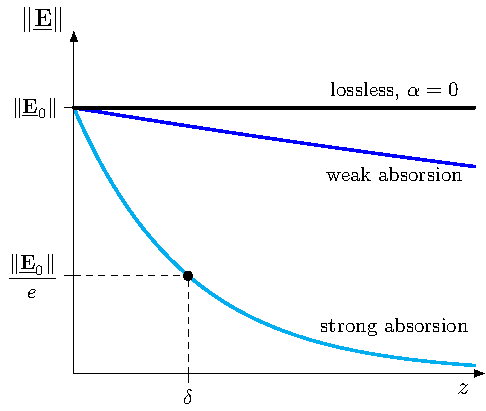
\includegraphics[width=\linewidth]{img/1/Skin-depth.pdf}
        \caption{Amplitude máxima de oscilação em função da distância de propagação~\protect\cite{silveirinha2023}. Escolheu-se $z$ para o exemplo.}
    \end{figure}
\end{minipage}\hfill
\begin{minipage}[b]{0.515\linewidth}
    O módulo da amplitude máxima de oscilação decai exponencialmente com a distância de propagação. Isto segue da definição em \eqref{eq:campos-onda-lossy-media}, onde $\mathbf{\underline{E}}_0$ é multiplicado pelos fatores
    \begin{equation*}
        e^{-\alpha \mathbf{\hat{d}} \cdot \mathbf{r}} \;\text{(regime exponencial)},
        \;\,
        e^{-j\beta \mathbf{\hat{d}} \cdot \mathbf{r}}
        \;\text{(regime sinusoidal)}.
    \end{equation*}
    O módulo $\norm{\mathbf{\underline{E}}}$ é obtido por:
    \begin{equation}
        \norm{\mathbf{\underline{E}}_0}\, e^{-\alpha \mathbf{\hat{d}} \cdot \mathbf{r}}
    \end{equation}
    Definimos a \emph{profundidade de penetração} (\emph{skin depth}) como:
    \begin{equation}
        \delta = \frac{1}{\alpha}
    \end{equation}
    A profundidade de penetração fornece uma estimativa aproximada da distância que uma onda pode penetrar dentro de um meio material antes de ser praticamente absorvida (i.e., decaia para ${\scriptsize \sim}37\%$ da amplitude original).
\end{minipage}


\begin{question}
    Para a frequência de oscilação de 1MHz, um material é caracterizado pela permitividade relativa $\epsilon_r = 2.5$ , pela permeabilidade relativa $\mu_r = 1$ , e pela condutividade $\sigma = 4 \times 10^{-5}$.\\[3pt]
    Determine: a) a tangente de perdas, b) a constante de atenuação, c) a constante de fase.
    
    \questionSep
    \textbf{Solução:} A tangente de perdas é definida em termos das partes real e imaginária da permitividade efetiva:
    $$
        \tan \theta = \frac{\epsilon''(\omega)}{\epsilon'(\omega)}\,\rightarrow\,
         \left\{
            \begin{aligned}
                &\epsilon'(\omega) =\epsilon_d'(\omega) = \epsilon_0\epsilon_r\\
                 &\epsilon''(\omega) =  \eqnmarkbox[violet]{pol-cunt}{\epsilon''_d(\omega)} + \frac{\sigma_c(\omega)}{\omega} = \frac{\sigma_c(\omega)}{\omega}
            \end{aligned}\right.
    $$
    \annotate[yshift=-0.1em]{below, label above}{pol-cunt}{Omitimos a componente da polarização}

    Assim,

    \vspace{-1.5em}
    $$
        \boxed{\tan \theta = \frac{\sigma}{\omega \epsilon_0 \epsilon_r} = 0.288}
    $$
    Ainda, $\gamma = jk = \alpha + j\beta$, logo:
    $$
        \begin{aligned}
            k = \omega\sqrt{\mu(\omega)\epsilon(\omega)} = \sqrt{\mu(\omega)\epsilon_d'(\omega)}\cdot\sqrt{1 - j\tan \theta} &= 0.0334 - j4.7\times 10^{-3} \; [\text{m}^{-1}]\\
            \gamma = jk &= \eqnmarkbox[violet]{fuck-waffle}{4.7\times 10^{-3} + j0.0334}
        \end{aligned}
    $$
    \annotate[yshift=-0.1em]{below, label above}{fuck-waffle}{$\alpha + j\beta$, respetivamente}
\end{question}
%//==============================--@--==============================//%
\clearpage
\subsubsection{Bons condutores e Bons Dielétricos}
Consideremos a dispersão de $\epsilon(\omega)$ e $\mu(\omega)$ negligenciável de forma a podermos escrever a constante de propagação e a impedância intrínseca da onda da seguinte forma:
\begin{align}
        \gamma &= j\omega\sqrt{\mu\left(\epsilon + \frac{\sigma}{j\omega}\right)} = j\omega\sqrt{\mu\epsilon}\eqnmarkbox[blue]{tan1}{\sqrt{1+\frac{\sigma}{j\omega\epsilon}}}\label{eq:gamma-nd}\\
        \eta &= \sqrt{\frac{\mu}{\epsilon + \frac{\sigma}{j\omega}}} = \sqrt{\frac{\mu}{\epsilon}}\frac{1}{\eqnmarkbox[blue]{tan2}{\sqrt{1+\frac{\sigma}{j\omega\epsilon}}}}\label{eq:eta}
\end{align}

\annotatetwo[yshift=-1cm,xshift=0cm]{below,right, label below}{tan1}{tan2}{Tanto a impedância quanto a constante de propagação\\ são governadas pelo parâmetro $\sqrt{1+\frac{\sigma}{j\omega\epsilon}}$}

\vspace{1.1em}
\begin{itemize}
    \item Caso $\sigma = 0$ o material torna-se não dispersivo e é dito \textit{dielétrico perfeito}.

    \item Caso $\sigma \neq 0$ mas $\sigma/\omega\epsilon \ll 1$ o material é dito \textit{bom dielétrico}. \eqref{eq:gamma-nd} e \eqref{eq:eta} podem ser escritas como
    \begin{equation}
        \gamma_{\text{good dielectric}} \approx \boxed{\dfrac{\sigma}{2}\sqrt{\frac{\mu}{\epsilon}} + j\frac{\omega}{c_0}\sqrt{\mu_r\epsilon_r}}\quad
        \eta_{\text{good dielectric}} \approx \boxed{\sqrt{\frac{\mu}{\epsilon}}\left(1+j\frac{\sigma}{2\omega\epsilon}\right)}
    \end{equation}

    \item Caso $\sigma/\omega\epsilon \gg 1$ o material é dito \textit{bom condutor} e: 
    \begin{equation}
        \gamma_{\text{good conductor}} \approx \boxed{\sqrt{\frac{\sigma\omega\mu}{2}}(1+j)}\qquad
        \eta_{\text{good conductor}} \approx \boxed{\sqrt{\frac{\omega\mu}{2\sigma}}(1+j)}
    \end{equation}
\end{itemize}

\vspace{-1em}
\begin{question}
    Um forno de micro-ondas trabalha à frequência de 2.5GHz. Nesta frequência um bife de lombo tem a permitividade complexa $30(1 - j0.3)\epsilon_0$.\\[3pt] 
    a) Qual o comprimento das micro-ondas no bife?\\[3pt] 
    b) Qual a profundidade de penetração (pelicular) das micro-ondas no bife?\\[3pt] 
    c) Se o bife é colocado num prato de plástico com $\epsilon=(1.1-j2\times10^{-4})\epsilon_0$ e espessura $3$mm, explique como este procedimento afeta o aquecimento do bife pelas micro-ondas.
    
    \questionSep
    \textbf{Solução}: Admitimos que:

    \vspace{-1.5em}
    $$
        \lambda = \frac{2\pi}{\beta}\qquad \beta = \Re\{k\}
    $$
    Por sua vez, recorrendo ao cálculo de $k$, para o qual $k = \beta - j\alpha$ (por definição)
    $$
        k = \omega\sqrt{\mu(\omega)\epsilon(\omega)}
        = \omega\sqrt{\mu_0\cdot 30(1 - j0.3)\epsilon_0} = 289.89 - j42.55
    $$
    Finalmente:

    \vspace{-1.5em}
    $$
        \lambda = \frac{2\pi}{\beta} = 21.67\,\text{mm}
    $$
    A profundida de penetração é dada por:

    \vspace{-1em}
    $$
        \delta = \frac{1}{\alpha} = 2.35\,\text{cm}
    $$
    Assumindo agora que $\epsilon=(1.1-j2\times10^{-4})\epsilon_0$ admitimos que
    $$
        \tan\theta = \frac{\sigma}{\omega\epsilon} = \frac{2\times 10^{-3}}{1.1} \ll 1\quad \text{(bom dielétrico)}\;\rightarrow\;
         \left\{
            \begin{aligned}
                 \gamma &\approx \eqnmarkbox[violet]{gamma}{\frac{\sigma}{2}\sqrt{\frac{\mu}{\epsilon}} + j\frac{\omega}{c_0}\sqrt{\mu_r\epsilon_r}}\\
                 \delta &= \frac{1}{\alpha} = 200\,\text{m}
            \end{aligned}\right.
    $$
    \annotate[yshift=2mm]{above, label above}{gamma}{$\alpha + j\beta,\;\alpha = 5\times10^{-3}$}

    Como o prato possui apenas 3 mm e $\delta = 200$m. A dissipação de energia é negligenciável, i.e, há baixa absorção/reflexão de energia pelo prato. O procedimento não afeta significativamente o aquecimento do bife.
\end{question}
%//==============================--@--==============================//%
\clearpage
\subsection{Polarização das Ondas}

Uma oscilação do campo eletromagnético não é totalmente determinada pela amplitude do campo. Devido à natureza vetorial do campo, existe um grau de liberdade adicional relacionado com a direção do espaço ao longo da qual o campo oscila. Este grau de liberdade é conhecido como a \emph{polarização do campo}.

A curva fechada determinada pela evolução temporal de $\mathbf{E}(t) = \Re\{ \mathbf{\underline{E}}e^{j\omega t} \}$. num ciclo completo de tempo (com período $T = 2\pi / \omega$) é a \emph{curva de polarização}. É simples demonstrar que a curva de polarização é sempre planar, uma vez que está no plano gerado pelos vetores ortogonais $\mathbf{E'} = \Re\{ \mathbf{\underline{E}} \}$ e $\mathbf{E''} = \Im\{ \mathbf{\underline{E}} \}$.

As propriedades de polarização da onda plana são determinadas pelas magnitudes relativas e fases das constantes complexas $\underline{A}$ e $\underline{B}$. Escrevendo-as nas suas formas polares $\underline{A} = A e^{j\phi_A}$ e $\underline{B} = B e^{j\phi_B}$, onde $A$ e $B$ são magnitudes positivas, obtemos:
\begin{equation}
    \begin{aligned}
        \mathbf{\underline{E}} &= \bigl(\underline{A} \mathbf{\hat{y}} + \underline{B} \mathbf{\hat{x}}\bigl)e^{-jkz}\\
        &= \left[A e^{j\phi_A}\mathbf{\hat{y}} + B e^{j\phi_B}\mathbf{\hat{x}}\right]e^{-jkz}
    \end{aligned}
\end{equation}

Extraindo a parte real e definindo $\mathbf{E}(z,t) = \Re\{\mathbf{\underline{E}}e^{j\omega t}\} = E_x(z,t) \mathbf{\hat{x}} + E_y(z,t) \mathbf{\hat{y}}$, encontramos as componentes reais em $x$ e $y$:
\begin{equation}
    \begin{aligned}
        E_y(z,t) &= A \cos(\omega t - kz + \phi_A)\\
        E_x(z,t) &= B \cos(\omega t - kz + \phi_B)
    \end{aligned}
\end{equation}
Para determinar a polarização da onda, consideramos a dependência temporal destes campos num ponto fixo ao longo do eixo $z$, digamos em $z = 0$:
\begin{equation}
    \begin{aligned}
        E_y(t) &= A \cos(\omega t + \phi_A)\\
        E_x(t) &= B \cos(\omega t + \phi_B)
    \end{aligned}
\end{equation}
Definimos a fase relativa $\phi = \phi_A - \phi_B$. Após alguma manipulação algébrica obtemos uma equação quadrática para as componentes $E_x$ e $E_y$, que descreve uma elipse no plano $E_x,\,E_y$:
\begin{equation}
    \left( \frac{E_y(t)}{B} \right)^2 \sin^2 \phi_A + \left( \frac{E_x(t)}{A} \right)^2 \sin^2 \phi_B - 2 \cos \phi \frac{E_x(t)E_y(t)}{AB} = \sin^2 \phi
\end{equation}

A trajetória do campo obtém-se através da omissão de $t$. A expressão  é simplificada para% fofinho, estou aqui
\begin{equation}\label{eq:polarization-eq} 
     \eqnmarkbox[blue]{pol}{\frac{E_x^2}{A^2} + \frac{E_y^2}{B^2} - 2 \cos \phi\, \frac{E_xE_y}{AB} = \sin^2 \phi}
\end{equation}
\annotate[yshift=-0.5em]{below, label above}{pol}{Elipse de polarização}

\begin{check}
    Dependendo dos valores das três quantidades ${A, B, \phi}$, esta elipse de polarização pode ser uma elipse, um círculo ou uma linha reta. 

    \begin{figure}[H]
        \centering
        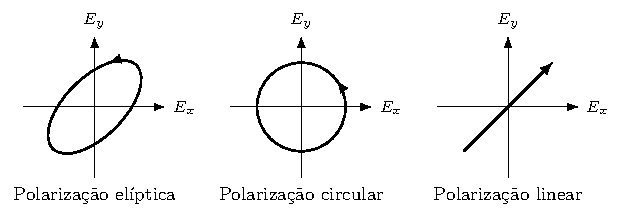
\includegraphics[width=0.75\linewidth]{img/1/Polarization.pdf}
        \caption{Tipos de polarização.}
    \end{figure}
\end{check}
%//==============================--@--==============================//%
\clearpage
Para obter a \textit{polarização linear}, definimos $\phi = 0$ ou $\phi = \pi$, o que corresponde a $\phi_A = \phi_B = 0$ ou $\phi_A = 0, \phi_B = -\pi$, de modo que as amplitudes dos fasores sejam $\mathbf{\underline{E}}_0 = \mathbf{\hat{y}}\underline{A} \pm \mathbf{\hat{x}}\underline{B}$. A Eq. \eqref{eq:polarization-eq} degenera em:
\begin{equation}
    \dfrac{E_{x}^2}{B^2} + \dfrac{E_{y}^2}{A^2} \pm \dfrac{2E_{x}E_{y}}{AB} = 0\,\rightarrow\, 
    \boxed{\left(\dfrac{E_{x}}{B} + \dfrac{E_{y}}{A}\right)^2 = 0}
\end{equation}
e consequentemente,
\begin{equation}
    \eqnmarkbox[blue]{lin}{E_{y} = \pm \dfrac{A}{B}E_{x}}
\end{equation}
\annotate[yshift=-0.1em]{below, label above}{lin}{reta de declive $\pm B/A$}

Para obter \textit{polarização circular}, definimos $A = B = R$ e $\phi = \pm \pi/2$. Neste caso, a elipse de polarização torna-se a equação de uma circunferência:
\begin{equation}
    \frac{E_{x}^2}{B^2} + \frac{E_{y}^2}{A^2} = 1
    \implies \eqnmarkbox[blue]{circ}{E_{x}^2 + E_{y}^2 = R^2}
\end{equation}
O sentido de rotação, em conjunto com a direção de propagação, define a polarização circular à esquerda/direita. Para o caso, $ \phi_a = -\pi/2 $ e $ \phi_b = 0 $, temos $\phi = \phi_a - \phi_b = -\pi/2$ e amplitude complexa $ \mathbf{\underline{E}}_0 = A(\mathbf{\hat{x}} - j\mathbf{\hat{y}}) $.

\vspace{-0.75em}
\begin{minipage}[c]{0.3\linewidth}
    \begin{figure}[H]
        \centering
        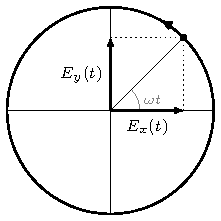
\includegraphics[width=0.915\linewidth]{img/1/Circular-polarization.pdf}
        \caption{Polarização circular.}
    \end{figure}
\end{minipage}\hfil
\begin{minipage}[c]{0.65\linewidth}
    Então,
     \begin{equation*}
        \begin{aligned}
            E_{x}(t) &= A \cos(\omega t)\\
            E_{y}(t) &= A \cos(\omega t - \pi/2) = A \sin(\omega t)
        \end{aligned}
    \end{equation*}
    Para determinar o sentido de rotação recorremos à evolução temporal do campo elétrico na curva de polarização. Calculando $\mathbf{E}(t=0)$ e $\mathbf{E}(t=0^+)$:
    \begin{equation*}
        t = 0: \, \left\{
        \begin{aligned}
            E_{x}(0) &= A\\
            E_{y}(0) &= 0
        \end{aligned}\right.
        \qquad
        t = 0^+: \, \left\{
        \begin{aligned}
            E_{x}(0^+) &\approx A\\
            E_{y}(0^+) &\approx 0^+
        \end{aligned}\right.
    \end{equation*}
    O campo gira no sentido anti-horário no plano $xy$.
\end{minipage}

\begin{warning}
    Para decidir se a polarização circular é à direita ou à esquerda, usamos a convenção da IEEE~\cite{ieee1983terms}: 
    \begin{itemize}
        \item Enrolar os dedos da mão esquerda e direita em punho e apontar ambos os polegares na direção de propagação. 
        \item Se os dedos da mão direita (esquerda) enrolam na direção de rotação do campo elétrico, então a polarização é à direita (esquerda).
    \end{itemize}
    Portanto, neste exemplo, como o campo se move na direção de $z$ e gira no sentido anti-horário, a polarização será à direita.
\end{warning}

Caso $A \neq B$ e $\phi = \pm \pi/2$, obtemos uma \textit{polarização elíptica}\footnote{A análise da orientação da polarização é análoga à da polarização circular.}. A Eq. \eqref{eq:polarization-eq} será agora:
\begin{equation}
    \eqnmarkbox[blue]{eli}{\frac{E_{x}^2}{B^2} + \frac{E_{y}^2}{A^2} = 1}
\end{equation}

\subsubsection{Rácio de Polarização}

Em resumo, definindo a amplitude complexa $\mathbf{\underline{E}} = \underline{E}_1 \mathbf{\hat{u}}_1 + \underline{E}_2 \mathbf{\hat{u}}_2$, tal que o par de versores ($\mathbf{\hat{u}}_1$, $\mathbf{\hat{u}}_2$) forme uma base ortogonal do plano perpendicular à direção de propagação $\mathbf{\hat{d}} = \mathbf{\hat{u}}_1 \times \mathbf{\hat{u}}_2$, podemos estabelecer o \textit{rácio de polarização}:
\begin{equation}
    p = \frac{\underline{E}_2}{\underline{E}_1} \equiv \abs{p} e^{j\phi}
\end{equation}

\begin{check}
    A amplitude $\abs{p}$ e a fase $\phi$ da razão de polarização determinam completamente a polarização da onda de acordo com as seguintes regras:
    \begin{itemize}
        \item Se $\phi = \pm \pi/2$ e $\abs{p} = 1$, a onda tem polarização circular.
        \item Se $\phi = 0$ ou $\phi = \pi$ ou $\abs{p} = 0$ ou $\abs{p} = \infty$, a onda tem polarização linear.
        \item Se nenhuma das condições acima se verifica, então o estado de polarização é elíptico.
    \end{itemize}
    Além disto, o ângulo $\phi$ controla o sentido de rotação, de modo que para $0 < \phi < \pi$ a onda está polarizada para a esquerda, enquanto para $-\pi < \phi < 0$ a onda está polarizada para a direita. É de sublinhar que este resultado só é válido quando a direção de propagação é $\mathbf{\hat{d}} = \mathbf{\hat{u}}_1 \times \mathbf{\hat{u}}_2$.
\end{check}

A mesma análise poderá ser feita com o campo $\mathbf{H}$, naturalmente.

%//==============================--@--==============================//%
\vfill
\begin{question}
    O fasor do campo magnético associado a uma onda plana e uniforme é dado por:
    $$
        \mathbf{\underline{H}} = \frac{10^{-3}}{120\pi}\left(\mathbf{\hat{x} - j\mathbf{\hat{y}}}\right)e^{jky}
    $$
    a) Determine o estado de polarização da onda.\\[3pt]
    b) Diga qual o sentido de rotação.\\[3pt]
    c) Esboce a curva de polarização.

    \questionSep
    \textbf{Solução}: Extraindo a parte real e definindo $\mathbf{H}(y,t) = \Re\{\mathbf{\underline{H}} e^{j\omega t}\} = H_x(y,t) \mathbf{\hat{x}} + H_z(y,t) \mathbf{\hat{z}}$, encontramos as componentes reais em $x$ e $y$:
    \begin{equation}
        \begin{aligned}
            H_z(y,t) &= \frac{10^{-3}}{120\pi} \cos\left(\omega t + ky -\pi/2\right)\\[1pt]
            H_x(y,t) &= \frac{10^{-3}}{120\pi} \cos(\omega t + ky)
        \end{aligned}
    \end{equation}
    Para determinar a polarização da onda, consideramos a dependência temporal do campo num ponto fixo ao longo do eixo $y$, digamos em $y = 0$:
    \begin{equation}
        \begin{aligned}
            H_z(t) &= \frac{10^{-3}}{120\pi} \cos\left(\omega t -\pi/2\right) = \frac{10^{-3}}{120\pi}\sin(\omega t)\\[1pt]
            H_x(t) &= \frac{10^{-3}}{120\pi} \cos(\omega t)
        \end{aligned}
    \end{equation}
    Como $\phi = 0 - (-\pi/2) = \pi/2$ a equação de polarização é dada por:
    $$
       H_{x}^2 + H_{z}^2 = 10^{-6}/(120\pi)^2\quad \text{(Polarização circular)}
    $$
    Para determinar o sentido de rotação recorremos à evolução temporal do campo elétrico na curva de polarização. Calculando $\mathbf{H}(t=0)$ e $\mathbf{H}(t=0^+)$:
    \begin{equation*}
        t = 0: \, \left\{
        \begin{aligned}
            H_{x}(0) &= \frac{10^{-3}}{120\pi}\\[1pt]
            H_{z}(0) &= 0
        \end{aligned}\right.
        \qquad
        t = 0^+: \, \left\{
        \begin{aligned}
            H_{x}(0^+) &\approx \frac{10^{-3}}{120\pi}\\[1pt]
            H_{z}(0^+) &\approx 0^+
        \end{aligned}\right.
    \end{equation*}
    O campo gira no sentido anti-horário no plano $xz$. A polarização é à direita por congruência com a regra da mão direita (nomeadamente, os dedos da mão direita enrolam na direção de rotação do campo magnética, com o polegar a apontar na direção de propagação).
    
    \qed
\end{question}
%//==============================--@--==============================//%
        %//==============================--@--==============================//%
\clearpage
\section{Energia Eletromagnética e o Vetor de Poynting}

As ondas eletromagnéticas transportam potência eletromagnética. A energia é transportada através do espaço até pontos recetores distantes por meio de ondas eletromagnéticas.

Consideremos um volume $V$ delimitado pela sua superfície de fronteira $\Sigma$. A região dentro de $V$ contém materiais arbitrários. O volume poderá conter fontes de campo modeldas por uma densidade de corrente externa $\mathbf{J}$. Definiremos $\mathcal{E}_{EM}$ como a energia armazenada no campo eletromagnético no volume $V$ e no instante $t$:
\begin{equation}
    \frac{d\mathcal{E}_{EM}}{dt} = \mathcal{P}_{ext} - \mathcal{P}_{dis} - \mathcal{P}_{\Sigma}
\end{equation}
\begin{itemize}
    \item $\mathcal{P}_{ext}$ descreve a potência injetada no volume $V$ (contribui para o aumento de energia em $V$).
    \item $\mathcal{P}_{dis}$ descreve a energia dissipada (por unidade de tempo) nos materiais na forma de calor.
    \item $\mathcal{P}_{\Sigma}$ descreve o fluxo de potência de $V$ para o exterior através da fronteira $\Sigma$ (caso positivo $[$negativo$]$, existe um fluxo de energia a sair do $[$entrar no$]$ volume $V$).
\end{itemize}

%//==============================--@--==============================//%
\subsection{Potência injetada}
Consideremos agora uma carga pontual com velocidade $\mathbf{v}$. Na presença de um campo, a partícula está sujeita à força de Lorentz $\mathbf{F} = q(\mathbf{E} + \mathbf{v} \times \mathbf{B})$. A potência instantânea transferida do campo para a carga é dada por\footnote{O campo magnético não contribui para a potência porque a força magnética é sempre perpendicular à velocidade da partícula.} $\mathbf{F} \cdot \mathbf{v}$:
\begin{equation}
    \mathcal{P}_{\text{field}\rightarrow\text{charge}} = \mathbf{F} \cdot \mathbf{v} = q \mathbf{E}\cdot\mathbf{v}
\end{equation}
Admitindo um volume $dV$ na região fonte, a carga total dentro de $dV$ será dada por $dQ = \rho_{\text{ext}}\,dV$ onde ${\rho_\text{ext}}$ é a densidade de carga. A potência transferida das cargas em $dV$ para o campo é:
\begin{equation}\label{eq:power-trans}
    d\mathcal{P}_{\text{charge in dV}\rightarrow\text{field}} = -dQ\, \mathbf{E} \cdot \mathbf{v} = -dV\, \mathbf{E} \cdot \eqnmarkbox[blue]{jota}{\rho_{\text{ext}} \mathbf{v}}
\end{equation}
\annotate[yshift=-0.1em]{below, label above}{jota}{densidade de corrente}

A densidade de corrente e a densidade de carga relacionam-se mediante $\mathbf{J}_{ext} = \rho_{\text{ext}}\mathbf{v}$; é então possível reescrever \eqref{eq:power-trans} de modo a que $d\mathcal{P}_{\text{ext}} = -dV\, \mathbf{E}\cdot \mathbf{J}_{ext}$. A potência total transferida das fontes externas para o campo é:
\begin{equation}
    \mathcal{P}_{\text{charge in dV}\rightarrow\text{field}} \equiv \mathcal{P}_\text{ext}= -\int_V \mathbf{E} \cdot \mathbf{J}_{ext} \,dV
\end{equation}
%//==============================--@--==============================//%
\subsection{Teorema de Poynting}
Para obter a lei de conservação de energia é necessário avaliar a divergência de $\mathbf{E} \times \mathbf{H}$. Este vetor é denominado por \textit{vetor de Poynting} (letra $\mathbf{S}$), e é representado em unidades de $[$W/m$^2]$.
\begin{equation}
    \boxed{\mathbf{S} = \mathbf{E} \times \mathbf{H}}
\end{equation}
Recorrendo às equações de Maxwell macroscópicas, e assumindo materiais não dispersivos (para os quais $\mu$ e $\epsilon$ são independentes da frequência),% e desprezando a existência de correntes de condução (nomeadamente desprezando a energia dissipada em forma de calor):

\vspace{-1em}
\begin{align}
    \nabla \times \mathbf{E} &= -\mu\frac{\partial \mathbf{H}}{\partial t} \\[1pt]
    \nabla \times \mathbf{H} &= \mathbf{J}_{ext} + \sigma \mathbf{E} + \epsilon\frac{\partial \mathbf{E}}{\partial t}
\end{align}
e à seguinte identidade vetorial:
\begin{equation}
    \nabla \cdot (\mathbf{E} \times \mathbf{H}) = \mathbf{H} \cdot (\nabla \times \mathbf{E}) - \mathbf{E} \cdot (\nabla \times \mathbf{H})
\end{equation}
É possível obter:
\begin{equation}\label{eq:Poynting}
    \nabla \cdot (\mathbf{E} \times \mathbf{H}) = -\mu\left(\mathbf{H} \cdot \frac{\partial \mathbf{H}}{\partial t}\right) - \epsilon\left(\mathbf{E} \cdot \frac{\partial \mathbf{E}}{\partial t}\right) -\mathbf{E} \cdot \mathbf{J}_{ext} - \sigma \mathbf{E} \cdot \mathbf{E}
\end{equation}
Subsequentemente, recorrendo à regra da cadeia para a derivada,
\begin{equation}
    \mu \left( \mathbf{H} \cdot \frac{\partial \mathbf{H}}{\partial t} \right) = \frac{1}{2} \mu \frac{\partial}{\partial t}(\mathbf{H}^2), 
    \qquad
    \varepsilon \left( \mathbf{E} \cdot \frac{\partial \mathbf{E}}{\partial t} \right) = \frac{1}{2} \varepsilon \frac{\partial}{\partial t}(\mathbf{E}^2)
\end{equation}

A equação \eqref{eq:Poynting} pode então ser escrita como
\begin{equation}
    \nabla \cdot (\mathbf{E} \times \mathbf{H}) = -\frac{\partial}{\partial t} \eqnmarkbox[blue]{Work}{\left( \frac{1}{2} \varepsilon \mathbf{E}^2 + \frac{1}{2} \mu \mathbf{H}^2 \right)} -\mathbf{E} \cdot \mathbf{J}_{ext} - \sigma \mathbf{E} \cdot \mathbf{E}
\end{equation}
\annotate[yshift=-0.1em]{below, label above}{Work}{density of electromagnetic energy, $W_{\text{EM}}$}

A forma integral da equação acima é obtida integrando ambos os lados sobre o volume de interesse:
\begin{equation}
    \int_V \nabla\cdot(\mathbf{E} \times \mathbf{H}) \, dV =\int_V \nabla\cdot \mathbf{S} \, dV = -\frac{\partial}{\partial t} \int_V \left( \frac{1}{2} \varepsilon \mathbf{E}^2 + \frac{1}{2} \mu \mathbf{H}^2 \right) dV + \mathcal{P}_{ext} - \int_V \sigma (\mathbf{E} \cdot \mathbf{E}) \, dV
\end{equation}
Finalmente, recorrendo ao teorema da divergência, de modo a transformar o integral de volume num integral sobre a fronteira da superfície:
\begin{equation}
    \int_{V} \nabla \cdot \mathbf{S} \, dV = \int_{\Sigma} \mathbf{S} \cdot \mathbf{\hat{n}} \, dA
\end{equation}
onde $\mathbf{\hat{n}}$ é o vetor unitário normal à superfície e direcionado para o exterior de $V$. Combinando as duas últimas equações, obtemos o \textit{teorema de Poynting}:
\begin{equation}
        \boxed{%
            \frac{\partial}{\partial t} \int_{V} W_{\text{EM}} \, dV
            =
            \mathcal{P}_{ext} 
            - \int_{\Sigma} \mathbf{S} \cdot \mathbf{\hat{n}} \, dA 
            - \int_V \sigma (\mathbf{E} \cdot \mathbf{E}) \, dV
        }
\end{equation}
\begin{check}
    \vspace{1em}
    \begin{equation*}
        \eqnmarkbox[blue]{Poynting-energy-1}{\frac{\partial}{\partial t} \int_{V} W_{\text{EM}} \, dV} 
        = \mathcal{P}_{\text{ext}} 
        - \eqnmarkbox[red]{Poynting-flux-1}{\int_{\Sigma} \mathbf{S} \cdot \mathbf{\hat{n}} \, dA}
        - {\color{gray} \mathcal{P}_{dis}}
        \quad\qquad\quad  
        \eqnmarkbox[blue]{Poynting-energy-2}{\frac{\partial\mathcal{E}_{EM}}{\partial t}} 
        = 
        \mathcal{P}_{ext}  
        - \eqnmarkbox[red]{Poynting-flux-2}{\mathcal{P}_{\Sigma}}
        - {\color{gray} \mathcal{P}_{dis}}
    \end{equation*}
    \annotatetwo[yshift=1mm]{above, label below}{Poynting-energy-1}{Poynting-energy-2}{electromagnetic field energy}
    \annotatetwo[yshift=-2mm]{below, label above}{Poynting-flux-1}{Poynting-flux-2}{net power flowing through the boundary}

    \vspace{1em}
    O \textit{teorema de Poynting} afirma que a potência total que flui para \textit{dentro} de uma superfície fechada em qualquer instante de tempo é igual à soma das taxas de aumento das energias elétrica e magnética armazenadas e da potência injetada dentro do volume fechado. Caso se contabilizasse a energia dissipada, teríamos ainda o fator:
    \begin{equation*}
        \mathcal{P}_{dis} = \int_V \sigma (\mathbf{E} \cdot \mathbf{E}) \, dV
        \quad \text{(perdas em forma de calor devido a correntes de condução)}
    \end{equation*}
\end{check}

\begin{warning}
    $\mathbf{S}$ determina o fluxo de energia eletromagnética no espaço. Quando $\mathbf{S}$ é uniforme e perpendicular à superfície, a potência que atravessa a superfície $\Sigma$ é dada por:
    $$
        P_{\Sigma} = \norm{\mathbf{S}} \cdot A
    $$
    sendo $A$ a área da superfície. 
\end{warning}

%//==============================--@--==============================//%
\clearpage
\subsection{Vetor de Poynting em Regimes Harmónicos no Tempo}
Admitindo uma excitação harmónica no tempo, o campo elétrico pode ser expresso como:
\begin{equation}
    \mathbf{E} = \Re\{\mathbf{\underline{E}}e^{j\omega t}\} = \frac{1}{2}\left[\mathbf{\underline{E}}e^{j\omega t} + \mathbf{\underline{E}^*}e^{-\omega t}\right]
\end{equation}
Analogamente para o campo magnético:
\begin{equation}
    \mathbf{H} = \Re\{\mathbf{\underline{H}}e^{j\omega t}\} = \frac{1}{2}\left[\mathbf{\underline{H}}e^{j\omega t} + \mathbf{\underline{H}^*}e^{-\omega t}\right]
\end{equation}
Consequentemente o vetor de Poynting é dado por:
\begin{equation}
    \mathbf{S} = \mathbf{E} \times \mathbf{H} =
    \frac{1}{4}\left[\mathbf{\underline{E}}\times\mathbf{\underline{H}}^* + \mathbf{\underline{E}}^*\times\mathbf{\underline{H}}\right] + \frac{1}{4}\left[\mathbf{\underline{E}}\times\mathbf{\underline{H}}e^{j2\omega t} + \mathbf{\underline{E}}^*\times\mathbf{\underline{H}}^*e^{-j2\omega t}\right]
\end{equation}
O vetor de Poynting médio  é obtido através da sua integração ao longo de um período de oscilação.
\begin{equation}
    \mathbf{S}_\text{av} = \frac{1}{T}\int_0^T \mathbf{S}(t) \, dt  = \eqnmarkbox[red]{Poynting-time-harm}{\frac{1}{4} \left[\mathbf{\underline{E}}\times\mathbf{\underline{H}}^* + \mathbf{\underline{E}}^*\times\mathbf{\underline{H}}\right]}
\end{equation}
\annotate[yshift=-2mm]{below, label above}{Poynting-time-harm}{parcela independente do tempo,\\ não afetada pela integração}

 que também pode ser escrito como:
 \begin{equation}
    \mathbf{S}_\text{av} = \frac{1}{2} \text{Re} \{ \mathbf{\underline{E}} \times \mathbf{\underline{H}}^* \}
\end{equation}
O vetor de Poynting médio determina o fluxo de potência média. Assim, a potência média no tempo que atravessa uma certa superfície $\Sigma$ é dada por:
\begin{equation}
    \mathcal{P}_{\Sigma, \text{av}} = \int_{\Sigma} (\mathbf{S}_{\text{av}}\cdot\mathbf{\Hat{n}}) \, d\mathbf{A}.
\end{equation}

%//==============================--@--==============================//%
\subsection{Vetor de Poynting para Ondas Plana}

Para uma onda plana eletromagnética num meio isotrópico, temos:
\begin{equation}
    \mathbf{E} = \eta \mathbf{H} \times \mathbf{\hat{d}},\qquad
    \mathbf{H} = -\frac{1}{\eta} \mathbf{\hat{d}} \times \mathbf{E}.
\end{equation}
Assim, o vetor de Poynting médio (densidade de potência) pode ser expresso como:
\begin{equation}
    \mathbf{S}_\text{av} = \frac{1}{2} \Re \left\{ \mathbf{E} \times \left[-\frac{1}{\eta} \mathbf{\hat{d}} \times \mathbf{E}^* \right] \right\}.
\end{equation}

Usando a identidade vetorial $ \mathbf{A} \times (\mathbf{B} \times     \mathbf{C}) = \mathbf{B}(\mathbf{A} \cdot \mathbf{C}) - \mathbf{C}(\mathbf{A} \cdot \mathbf{B}) $ e recordando que o campo é transversal $ \mathbf{E} \cdot \mathbf{\hat{d}} = 0 $, descobre-se que
\begin{equation}
    \mathbf{S}_\text{av} = \frac{1}{2} \Re \left\{\mathbf{\hat{d}}\frac{1}{\eta^*}  \mathbf{E} \cdot \mathbf{E}^* \right\},
\end{equation}
o que também pode ser expresso como:
\begin{equation}
    \mathbf{S}_\text{av} = \frac{1}{2} \Re \left\{ \frac{1}{\eta} \right\}\norm{\mathbf{\underline{E}}}^2 \mathbf{\hat{d}} = \frac{1}{2} \Re \left\{\eta\right\} \norm{\mathbf{\underline{H}}}^2\mathbf{\hat{d}}
\end{equation}
Admitimos que $\Re \left\{  \frac{1}{\eta^*} \right\} = \Re \left\{ \frac{1}{\eta} \right\}$. A segunda identidade é uma consequência da relação $ |\mathbf{E}| = |\eta| |\mathbf{H}| $. Para materiais sem perdas, a impedância intrínseca é real e, portanto, o vetor de Poynting pode ser expresso como:
\begin{equation}
    \mathbf{S}_\text{av} = \frac{1}{2} \frac{1}{\eta}\norm{ \mathbf{\underline{E}}}^2 \mathbf{\hat{d}} = \frac{1}{2} \eta \norm{\mathbf{\underline{H}}}^2 \mathbf{\hat{d}}. \quad \text{(materiais sem perdas)}.
\end{equation}
O vetor de Poynting está alinhado com $\mathbf{\hat{d}}$. Assim, em materiais isotrópicos, a energia flui na direção de propagação da onda.% adoro-te 

\begin{question}
    Considere a onda plana descrita pelo fasor:
    $$
        \mathbf{\underline{E}} = E_0 \mathbf{\Hat{y}}e^{-jk_0z}
    $$
    a) Determine $\mathbf{S}$ e $\mathbf{S}_\text{av}$\\[3pt]
    b) Se $E_0 = 1$V/m determine a potência média que atravessa a superfície na figura abaixo:
    \begin{figure}[H]
        \centering
        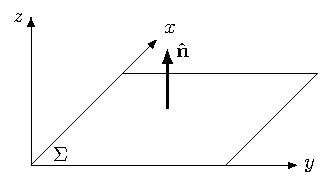
\includegraphics[width=0.3\linewidth]{img/1/Plane.pdf}
    \end{figure}

    \vspace{-1em}
    \questionSep
    \textbf{Solução:} Reconhecemos que:
    $$
        \mathbf{S} = \mathbf{E}\times\mathbf{H}
    $$
    O campo elétrico instantâneo pode ser calculado através de:
    $$
        \mathbf{E} = \Re\{\mathbf{\underline{E}} e^{j\omega t}\} = E_0\mathbf{\hat{y}}\cos(\omega\,t - k_0 z)
    $$
    e o campo magnético por:
    $$
        \begin{aligned}
             \eqnmarkbox[violet]{mag-field}{\mathbf{H}} = \frac{1}{\eta_0} \mathbf{\Hat{d}}\times \mathbf{E}
            &= \frac{E_0}{\eta_0} \eqnmarkbox[violet]{direction}{\mathbf{\Hat{z}}}\times\mathbf{\Hat{y}}\cos(\omega\,t - k_0 z)\\
            &= \boxed{-\frac{E_0}{\eta_0} \mathbf{\Hat{x}}\cos(\omega\,t - k_0 z)}
        \end{aligned}
    $$
    \annotate[yshift=1.5mm]{above, label above}{direction}{Por inspeção do fasor do campo elétrico, $\mathbf{\Hat{d}} = \mathbf{\Hat{z}}$}
    \annotate[yshift=-1.5mm]{below,left, label above}{mag-field}{Válido para meios sem perdas}
    
    Finalmente,
    $$
        \begin{aligned}
            \mathbf{S} &= -\frac{E_0}{\eta_0} \mathbf{\Hat{x}}\cos(\omega\,t - k_0 z)\times E_0\mathbf{\hat{y}}\cos(\omega\,t - k_0 z)\\
            &= \boxed{-\frac{E_0^2}{\eta_0} \mathbf{\Hat{z}}\cos(\omega\,t - k_0 z)^2}
        \end{aligned}
    $$
    O cálculo de $\mathbf{S}_{\text{av}}$ resulta em:
    $$
        \mathbf{S}_{\text{av}} = \frac{1}{2} \frac{1}{\eta_0}| \mathbf{\underline{E}}|^2
        = \frac{1}{2} \frac{1}{ \eqnmarkbox[violet]{imp}{\eta_0}}|E_0|^2
    $$
    \annotate[xshift=3mm,yshift=1mm]{below,right, label above}{imp}{$120\pi$}

    Por fim, a potência média que atravessa a superfície é dada por:
    $$
        \begin{aligned}
             \mathcal{P}_{\Sigma, \text{av}} = \int_{\Sigma} (\mathbf{S}_\text{av}\cdot\mathbf{\Hat{n}}) \, dA &= \norm{\mathbf{S}_\text{av}} \cdot A\\
             &= \frac{1}{2} \frac{1}{\eta_0}|E_0|^2\cdot A = \boxed{1.33\, \text{mW}}
        \end{aligned}
    $$
    Tal como explicitado na \hyperref[warn:6]{Nota 6}, sendo $\mathbf{S}$ uniforme e prependicular à superfície, o cálculo da potência média degenera no produto da norma do $\mathbf{S}_\text{av}$ com a área da superfície.
\end{question}% miminhos




%//==============================--@--==============================//%
        %//==============================--@--==============================//%
\clearpage
\section{Reflexão e Refração}

%//==============================--@--==============================//%
\subsection{Condições de Fronteira}
\label{sec:boundary-conditions-waves}

As condições de fronteira para os campos eletromagnéticos na interação entre dois meios materiais são dadas abaixo:

\begin{figure}[H]
    \centering
    \begin{minipage}[c]{0.25\linewidth}
        $$
            \boxed{%
                \begin{aligned}
                    \mathbf{E}_{1t} - \mathbf{E}_{2t} &= 0 \\
                    \mathbf{H}_{1t} - \mathbf{H}_{2t} &= \mathbf{J}_{s} \times \mathbf{\hat{n}} \\
                    \mathbf{D}_{1n} - \mathbf{D}_{2n} &= \rho_{s} \\
                    \mathbf{B}_{1n} - \mathbf{B}_{2n} &= 0
                \end{aligned}
            }
        $$
    \end{minipage}\hspace{1em}
    \begin{minipage}[c]{0.55\linewidth}
        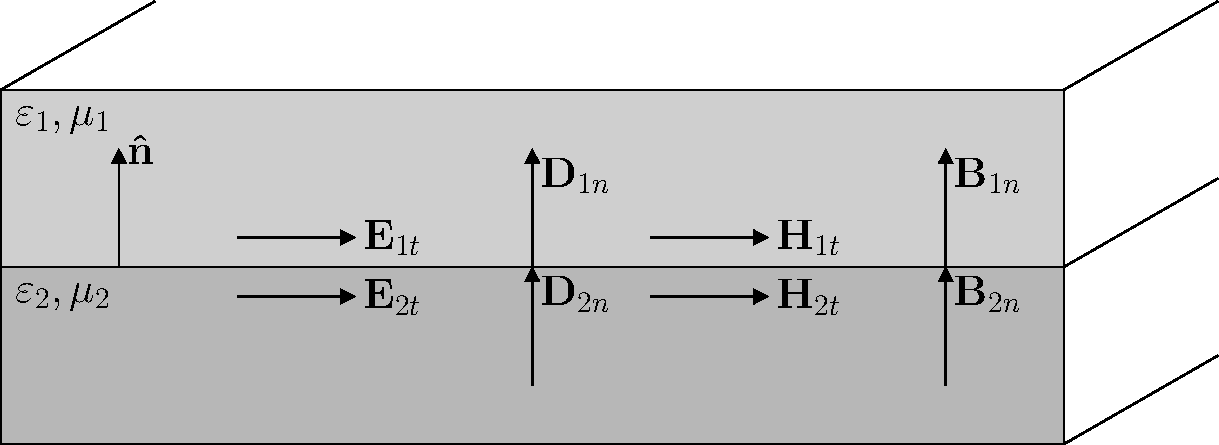
\includegraphics[width=0.925\linewidth]{img/1/Material-interface.pdf}
    \end{minipage}
    \caption{Condições de fronteira entre dois meios materiais}
    \label{fig:Material-interface}
\end{figure}

\vspace{-1em}
onde $\mathbf{\hat{n}}$ é um vetor unitário normal à fronteira (ou interface), que aponta do meio-2 para o meio-1.

As quantidades $\rho_s, \mathbf{J}_s$ são quaisquer \textit{cargas de superfície externas} e \textit{densidades de corrente de superfície} na superfície de fronteira e são medidas em unidades de $[\text{C/m}^2]$ e $[\text{A/m}]$.

Cada vetor pode ser decomposto como a soma de uma parte tangencial à superfície e uma parte perpendicular a ela, isto é, $\mathbf{E} = \mathbf{E}_t + \mathbf{E}_n$. Utilizando a identidade vetorial,
$$
    \mathbf{E} = \mathbf{\hat{n}} \times (\mathbf{E} \times \mathbf{\hat{n}}) + \mathbf{\hat{n}}(\mathbf{\hat{n}} \cdot \mathbf{E}) = \mathbf{E}_t + \mathbf{E}_n
$$
identificamos estas duas partes como:
$$
    \mathbf{E}_t = \mathbf{\hat{n}} \times (\mathbf{E} \times \mathbf{\hat{n}}), \quad \mathbf{E}_n = \mathbf{\hat{n}} (\mathbf{\hat{n}} \cdot \mathbf{E})
$$
Por outras palavras, as componentes \textit{tangenciais} do campo $\mathbf{E}$ são contínuas através da interface; a diferença das componentes \textit{tangenciais} do campo $\mathbf{H}$ são iguais às densidades de corrente da superfície; a diferença das componentes \textit{normais} da densidade de fluxo $\mathbf{D}$ são iguais à densidade de carga da superfície; e as componentes \textit{normais} da densidade de fluxo magnético $\mathbf{B}$ são contínuas.

\begin{warning}
    É relevante salientar que a continuidade dos campos tangenciais numa interface garante a continuidade da componente normal do vetor de Poynting na interface, se considerarmos $\mathbf{J}_{s} = 0$ temos:
    $$
        \mathbf{S}_1 \cdot \mathbf{\hat{n}} = (\mathbf{E}_1 \times \mathbf{H}_1) \cdot \mathbf{\hat{n}} = (\mathbf{E}_{1t} \times \mathbf{H}_{1t}) \cdot \mathbf{\hat{n}} = (\mathbf{E}_{2t} \times \mathbf{H}_{2t}) \cdot \mathbf{\hat{n}} = \mathbf{S}_2 \cdot \mathbf{\hat{n}}.
    $$
    Isto é, a interface não pode absorver a energia da onda.
\end{warning}

\begin{warning}
    É relevante analisar as condições de fronteira numa interface com um condutor elétrico perfeito (PEC)~\cite{silveirinha2023}. Um condutor elétrico perfeito é um material idealizado com condutividade elétrica $\sigma \to +\infty$. Como a corrente de condução é $\mathbf{J}_{\text{cond}} = \sigma \mathbf{E}$, o campo elétrico dentro de um condutor perfeito deve anular-se. Assim, um material PEC ideal comporta-se como um espelho perfeito e é impenetrável pela luz. Consequentemente, o campo elétrico na interface com um material PEC deve desaparecer:
    $$
        \mathbf{E}_{1t} = \mathbf{E}_{2t} = 0
        \quad \text{(interface PEC)}
    $$
    Note-se que o campo magnético tangencial $\mathbf{H}_{1t}$ (avaliado fora do material) não desaparece. Determina uma densidade de corrente de superfície na fronteira do PEC.
\end{warning}

%//==============================--@--==============================//%
\subsection{Incidência em Interfaces Planas}

Nesta secção focamos a nossa atenção na incidência de ondas planas em interfaces que separam dois meios materiais.

\subsubsection{Incidência Normal}

A direção de propagação da onda incidente, $\mathbf{\hat{d}}^i$, é perpendicular à superfície da interface. Nestes moldes, os campos da onda incidente são:
\begin{equation}
    \mathbf{\underline{E}}^{\text{inc}} = \mathbf{\underline{E}}^{\text{inc}}_{0}\, e^{-\gamma_1 \mathbf{\hat{d}}^i \cdot \mathbf{r}},
    \qquad
    \mathbf{\underline{H}}^{\text{inc}} = \frac{1}{\eta_1} \mathbf{\hat{d}}^i \times \mathbf{\underline{E}}^{\text{inc}}_{0}\, e^{-\gamma_1 \mathbf{\hat{d}}^i \cdot \mathbf{r}}
\end{equation}
através das relações apresentadas \ref{sec:ondas-com-perdas}.

\begin{figure}[H]
    \centering
    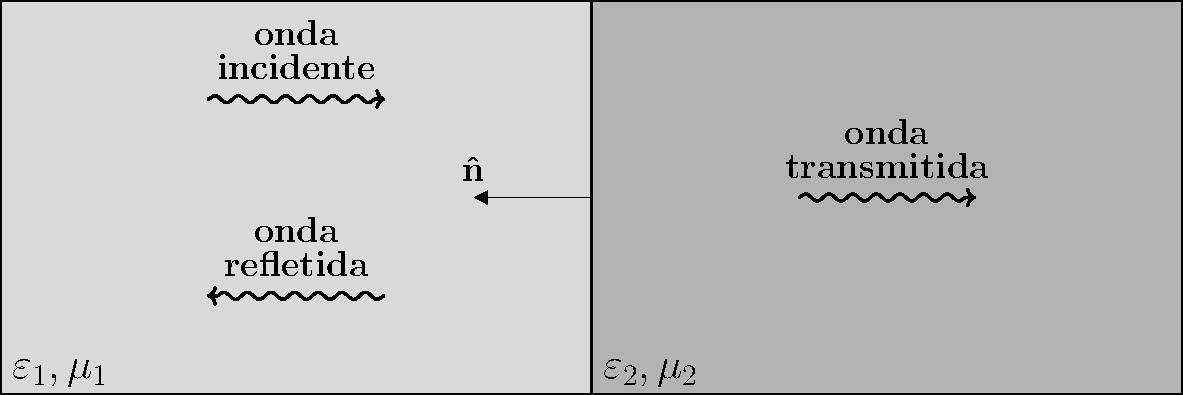
\includegraphics[width=0.5\linewidth]{img/1/Incidencia-normal.pdf}
    \caption{Incidência normal numa interface plana}
    \label{fig:Incidencia-normal}
\end{figure}

\vspace{-1em}
Como seria de esperar intuitivamente, a onda incidente irá gerar uma onda transmitida no meio 2 e uma onda refletida no meio 1, com direções de propagação $\mathbf{\hat{d}}^t = \mathbf{\hat{d}}^i$ e $\mathbf{\hat{d}}^r = -\mathbf{\hat{d}}^i$. Podemos escrever os campos respetivos:
\begin{equation}
    \mathbf{\underline{E}}^{\text{ref}} = \mathbf{\underline{E}}^{\text{ref}}_{0}\, e^{-\gamma_1 \mathbf{\hat{d}}^r \cdot \mathbf{r}},
    \qquad
    \mathbf{\underline{H}}^{\text{ref}} = \frac{1}{\eta_1} \mathbf{\hat{d}}^r \times \mathbf{\underline{E}}^{\text{ref}}_{0}\, e^{-\gamma_1 \mathbf{\hat{d}}^r \cdot \mathbf{r}}
\end{equation}
\begin{equation}
    \mathbf{\underline{E}}^{\text{tx}} = \mathbf{\underline{E}}^{\text{tx}}_{0}\, e^{-\gamma_2 \mathbf{\hat{d}}^t \cdot \mathbf{r}},
    \qquad
    \mathbf{\underline{H}}^{\text{tx}} = \frac{1}{\eta_1} \mathbf{\hat{d}}^t \times \mathbf{\underline{E}}^{\text{tx}}_{0}\, e^{-\gamma_2 \mathbf{\hat{d}}^t \cdot \mathbf{r}}
\end{equation}

Estes campos obdecem às condições de fronteira anunciadas \hyperref[sec:boundary-conditions-waves]{anteriormente}, uma vez que as ondas planas são transversais\footnote{Nesta situação, $\mathbf{\underline{E}}$ e $\mathbf{\underline{H}}$ são paralelos (tangenciais) à interface.}, i.e.,
\begin{equation}
    \begin{aligned}
        \mathbf{\underline{E}} =
        \begin{cases}
            \mathbf{\underline{E}}^{\text{inc}} + \mathbf{\underline{E}}^{\text{ref}} & \text{antes da interface} \\
            \mathbf{\underline{E}}^{\text{tx}} & \text{depois da interface}
        \end{cases}
        \qquad\quad
        \mathbf{\underline{H}} = 
        \begin{cases}
            \mathbf{\underline{H}}^{\text{inc}} + \mathbf{\underline{H}}^{\text{ref}} & \text{antes da interface} \\
            \mathbf{\underline{H}}^{\text{tx}} & \text{depois da interface}
        \end{cases}
    \end{aligned}
\end{equation}
que se reduz às relações:
\begin{equation} \label{eq:1.72}
    \mathbf{\underline{E}}^{\text{inc}} + \mathbf{\underline{E}}^{\text{ref}} = \mathbf{\underline{E}}^{\text{tx}},
    \qquad
    \frac{1}{\eta_1}\mathbf{\hat{d}}^i \times (\mathbf{\underline{E}}^{\text{inc}} - \mathbf{\underline{E}}^{\text{ref}}) = \frac{1}{\eta_2}\mathbf{\hat{d}}^i \times \mathbf{\underline{E}}^{\text{tx}}
\end{equation}
Removendo o produto externo da segunda relação, vem que
\begin{equation}
    \mathbf{\underline{E}}^{\text{inc}} + \mathbf{\underline{E}}^{\text{ref}} = \mathbf{\underline{E}}^{\text{tx}},
    \qquad
    \frac{1}{\eta_1} (\mathbf{\underline{E}}^{\text{inc}} - \mathbf{\underline{E}}^{\text{ref}}) = \frac{1}{\eta_2} \mathbf{\underline{E}}^{\text{tx}}.
\end{equation}
É conveniente definir a componente refletida e transmitida em função da componente incidente:
\begin{equation}
    \mathbf{\underline{E}}^{\text{ref}} = \rho \mathbf{\underline{E}}^{\text{inc}}
    \qquad
    \mathbf{\underline{E}}^{\text{tx}} = \tau \mathbf{\underline{E}}^{\text{inc}}
\end{equation}
onde $\rho$ é definido como coeficiente de reflexão e $\tau$ como coeficiente de transmissão. Da equação \ref{eq:1.72}, vem que
\begin{equation}
    \boxed{%
        \rho = \frac{\eta_2 - \eta_1}{\eta_1 + \eta_2}
    }
    \qquad\quad
    \boxed{%
        \tau = 1 + \rho = \frac{2\eta_2}{\eta_1 + \eta_2}
    }
\end{equation}
\textbf{Nota}: As componentes do campo são avaliadas na interface!

\begin{warning}
    \begin{itemize}
        \item  Quando as impedâncias dos dois materiais são idênticas ($\eta_2 = \eta_1$), não há onda refletida e a onda incidente é totalmente transmitida para o segundo meio. Neste caso, diz-se que os materiais estão ``adaptados''.
        
        \item A situação oposta ocorre quando o meio 2 é um condutor elétrico perfeito (PEC). Como a impedância intrínseca de um condutor perfeito desaparece ($\eta_{PEC} = \eta_2 = 0$), o coeficiente de reflexão nesse caso torna-se $\rho_{\text{PEC}} = -1$. Isso confirma que um condutor perfeito comporta-se como um espelho perfeito.    
    \end{itemize}
\end{warning}

%//==============================--@--==============================//%
\subsubsection{Incidência Oblíqua}

Numa situação mais geral, a onda incidente poderá atingir a interface numa direção oblíqua. Neste caso, é necessário ter em consideração o ângulo de incidência $\theta_i$, de reflexão $\theta_r$ e de transmissão $\theta_t$. Isto pode ser feito à custa do vetor unitário normal à interface, $\mathbf{\hat{n}}$.
\begin{equation}
    -\mathbf{\hat{d}}^i \cdot \mathbf{\hat{n}} = \cos \theta_i
    \qquad
    \mathbf{\hat{d}}^r \cdot \mathbf{\hat{n}} = \cos \theta_r
    \qquad
    \mathbf{\hat{d}}^t \cdot \mathbf{\hat{n}} = \cos \theta_t
\end{equation}
Definimos também o \emph{plano de incidência}, gerado pelos vetores $\mathbf{\hat{d}}^i$ e $\mathbf{\hat{n}}$.

\begin{figure}[H]
    \centering
    \begin{subfigure}[c]{0.55\linewidth}
        \centering
        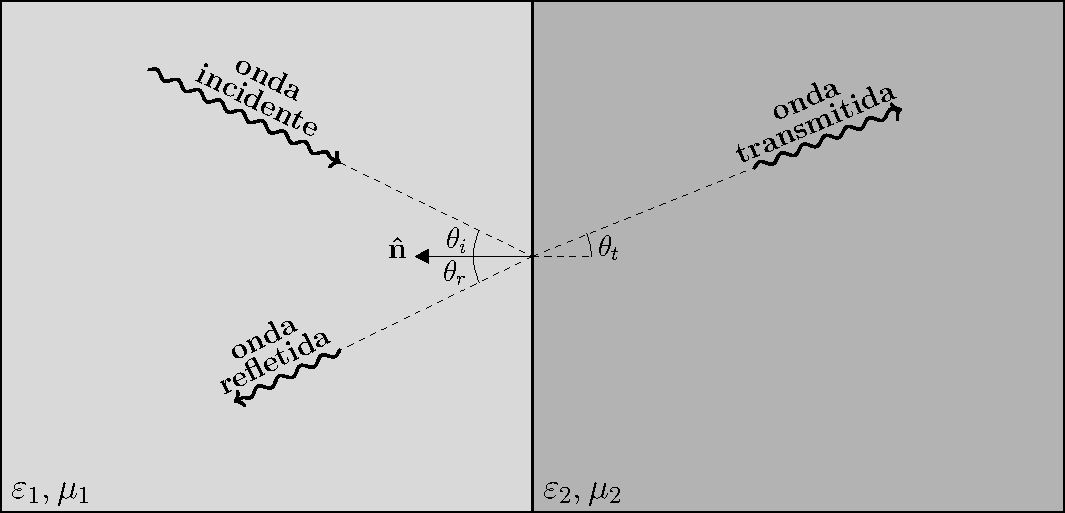
\includegraphics[width=\linewidth]{img/1/Incidencia-obliqua.pdf}
        \caption{Interação entre dois meios}
    \end{subfigure}\hfil
    \begin{subfigure}[c]{0.2\linewidth}
        \centering
        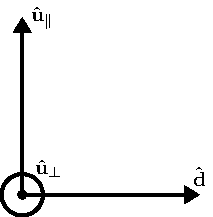
\includegraphics[width=\linewidth]{img/1/Vetores-unitarios.pdf}
        \caption{Relação entre os vetores unitários, $\mathbf{\hat{u}}_{\parallel} \times \mathbf{\hat{u}}_{\perp} = \mathbf{\hat{d}}$.}
    \end{subfigure}
    \caption{Incidência oblíqua numa interface plana}
    \label{fig:Incidencia-obliqua}
\end{figure}

\vspace{-1em}
Uma vez que os campos da onda incidente oscilam num plano transversal a $\mathbf{\hat{d}}^i$ ($\mathbf{E}^{\text{inc}} \cdot \mathbf{\hat{d}}^i = 0$), é conveniente introduzir dois vetores unitários, $\mathbf{\hat{u}}_{\parallel}$ e $\mathbf{\hat{u}}_{\perp}$, que geram este plano. Por construção, os vetores unitários cumprem a seguinte condição:
\begin{equation}
    \mathbf{\hat{u}}^{i}_{\parallel} \times \mathbf{\hat{u}}_{\perp} = \mathbf{\hat{d}}^i
\end{equation}
Note-se que o vetor $\mathbf{\hat{u}}_{\perp}$ é perpendicular ao plano de incidência, enquanto o vetor $\mathbf{\hat{u}}^{i}_{\parallel}$ é paralelo ao plano de incidência, de acordo com as notações. 

O campo incidente pode ser escrito em termos de $\mathbf{\hat{u}}_{\parallel}$ e $\mathbf{\hat{u}}_{\perp}$ da seguinte forma:
\begin{equation}
    \mathbf{\underline{E}}^{\text{inc}} = \underline{\mathrm{E}}^{i}_{\parallel} \mathbf{\hat{u}}^{i}_{\parallel} + \underline{\mathrm{E}}^{i}_{\perp} \mathbf{\hat{u}}_{\perp}
\end{equation}
onde as componentes $\underline{\mathrm{E}}^{i}_{\parallel}$ e $\underline{\mathrm{E}}^{i}_{\perp}$ são as componentes paralela e perpendicular do campo, respetivamente.

Uma construção similar pode ser feita para os campos $\mathbf{\underline{E}}^{\text{ref}}$ e $\mathbf{\underline{E}}^{\text{tx}}$,
\begin{equation}
    \mathbf{\hat{u}}^{r}_{\parallel} \times \mathbf{\hat{u}}_{\perp} = \mathbf{\hat{d}}^r
    \qquad\qquad
    \mathbf{\hat{u}}^{t}_{\parallel} \times \mathbf{\hat{u}}_{\perp} = \mathbf{\hat{d}}^t
\end{equation}
que leva às decomposições seguintes:
\begin{equation}
    \mathbf{\underline{E}}^{\text{ref}} = \underline{\mathrm{E}}^{r}_{\parallel} \mathbf{\hat{u}}^{r}_{\parallel} + \underline{\mathrm{E}}^{r}_{\perp} \mathbf{\hat{u}}_{\perp}
    \qquad\qquad
    \mathbf{\underline{E}}^{\text{tx}} = \underline{\mathrm{E}}^{t}_{\parallel} \mathbf{\hat{u}}^{t}_{\parallel} + \underline{\mathrm{E}}^{t}_{\perp} \mathbf{\hat{u}}_{\perp}
\end{equation}

%//==============================--@--==============================//%
\subsubsection{Lei de Snell}
\label{subsubsec:lei-de-snell}

Nesta secção viramos a nossa atenção para o ângulo de incidência $\theta_i$ e o ângulo de transmissão $\theta_t$. Podemos relacionar estes ângulos através das \hyperref[sec:boundary-conditions-waves]{condições de fronteira} já enunciadas.

Os campos associados às ondas planas incidentes, refletidas e transmitidas são:
\begin{equation}
    \mathbf{\underline{E}}^{\text{inc}} = \mathbf{\underline{E}}^{\text{inc}}_{0}\, e^{-\gamma_1 \mathbf{\hat{d}}^i \cdot \mathbf{r}}
    \qquad
    \mathbf{\underline{E}}^{\text{ref}} = \mathbf{\underline{E}}^{\text{ref}}_{0}\, e^{-\gamma_1 \mathbf{\hat{d}}^r \cdot \mathbf{r}}
    \qquad
    \mathbf{\underline{E}}^{\text{tx}} = \mathbf{\underline{E}}^{\text{tx}}_{0}\, e^{-\gamma_2 \mathbf{\hat{d}}^t \cdot \mathbf{r}}
\end{equation}
Impõe-se a continuidade das componentes do campo tangentes à interface e verifica-se que:
\begin{equation}
    \left[ \mathbf{\underline{E}}^{\text{inc}} + \mathbf{\underline{E}}^{\text{ref}} \right] \cdot \mathbf{\hat{t}} = \mathbf{\underline{E}}^{\text{tx}} \cdot \mathbf{\hat{t}}
    \quad\iff\quad
    \left[ \mathbf{\underline{E}}_{0}^{\text{inc}} e^{-\gamma_1 \mathbf{\hat{d}}^i \cdot \mathbf{r}} + \mathbf{\underline{E}}_{0}^{\text{ref}} e^{-\gamma_1 \mathbf{\hat{d}}^r \cdot \mathbf{r}} - \mathbf{\underline{E}}_{0}^{\text{tx}} e^{-\gamma_2 \mathbf{\hat{d}}^t \cdot \mathbf{r}} \right] \cdot \mathbf{\hat{t}} = 0.
\end{equation}
onde $\mathbf{\hat{t}}$ é uma direção genérica paralela à interface. Esta relação deve ser válida para qualquer ponto $\mathbf{r}$ da interface, ou seja, os fatores de fase devem ser iguais entre si:
\begin{equation}
    \gamma_1 \mathbf{\hat{d}}^i \cdot \mathbf{r} = \gamma_1 \mathbf{\hat{d}}^r \cdot \mathbf{r} = \gamma_2 \mathbf{\hat{d}}^t \cdot \mathbf{r},
\end{equation}
e assim $\mathbf{\hat{d}}^i$, $\mathbf{\hat{d}}^r$ e $\mathbf{\hat{d}}^t$ devem estar todos no mesmo plano, i.e., devem estar no plano de incidência $[$1\textordfeminine{} Lei de Snell$]$.

Podemos escrever a relação de continuidade para as componentes tangenciais em termos dos ângulos de incidência, reflexão e transmissão. A projeção de $\mathbf{\hat{d}}^i$, $\mathbf{\hat{d}}^r$ e $\mathbf{\hat{d}}^t$ na interface é $\sin \theta_i$, $\sin \theta_r$, e $\sin \theta_t$, respetivamente, de onde resulta
\begin{equation}
    \gamma_1 \sin \theta_i = \gamma_1 \sin \theta_r = \gamma_2 \sin \theta_t
\end{equation}
Esta relação pode ser reescrita sob a forma da 2\textordfeminine{} Lei de Snell (reflexão e refração):
\begin{equation}
    \boxed{%
        \theta_i = \theta_r
    },
    \qquad
    \boxed{%
        n_1 \sin \theta_i = n_2 \sin \theta_t
    },
    \; \text{onde $n_1 = \sqrt{\epsilon_{r1} \mu_{r1}}$ e $n_2 = \sqrt{\epsilon_{r2} \mu_{r2}}$}.
\end{equation}

%//==============================--@--==============================//%
\subsection{Polarização das Ondas Refletidas e Transmitidas}

Na incidência oblíqua (ou normal), a polarização das ondas refletidas e transmitidas altera-se em relação à incidente, podendo mudar de circular para elíptica e inverter a rotação.

Existem dois estados de polarização específicos (\textit{eigen-polarization}) --- paralelo e perpendicular ao plano de incidência --- que se conservam após a interação com a interface. Caso a onda incidente seja polarizada paralela ou perpendicularmente, as ondas refletidas e transmitidas mantêm essa característica, correspondendo, respetivamente, às polarizações magnética transversal (TM) e elétrica transversal (TE).

Uma onda incidente genérica pode ser considerada como a sobreposição de uma onda com polarização paralela e uma onda com polarização perpendicular. Assim, podemos escrever os campos como:
\begin{equation}
    \boxed{%
        \begin{aligned}
            \mathbf{\underline{E}}^{\text{inc}} &= \left( \underline{E}_{0\parallel}^i \mathbf{\hat{u}}_{\parallel} + \underline{E}_{0\perp}^i \mathbf{\hat{u}}_{\perp} \right) e^{-\gamma_1 \mathbf{\hat{d}}^i \cdot \mathbf{r}}, \\
            \mathbf{\underline{E}}^{\text{ref}} &= \left( \rho_{\parallel}\, \underline{E}_{0\parallel}^i \mathbf{\hat{u}}^{r}_{\parallel} + \rho_{\perp}\, \underline{E}_{0\perp}^i \mathbf{\hat{u}}_{\perp} \right) e^{-\gamma_1 \mathbf{\hat{d}}^r \cdot \mathbf{r}}, \\
            \mathbf{\underline{E}}^{\text{tx}} &= \left( \tau_{\parallel}\, \underline{E}_{0\parallel}^i \mathbf{\hat{u}}^{t}_{\parallel} + \tau_{\perp}\, \underline{E}_{0\perp}^i \mathbf{\hat{u}}_{\perp} \right) e^{-\gamma_2 \mathbf{\hat{d}}^t \cdot \mathbf{r}}.
        \end{aligned}
    }
\end{equation}
Sem perda de generalidade, supõe-se que a origem do sistema de coordenadas está contida na interface do material.

Para a componente polarizada \underline{paralelamente} ($\parallel$), o coeficiente de reflexão e o coeficiente de transmissão são:
\begin{equation}
    \rho_{\parallel} = \frac{\eta_1 \cos \theta_i - \eta_2 \cos \theta_t}{\eta_1 \cos \theta_i + \eta_2 \cos \theta_t},
    \qquad
    \tau_{\parallel} = \frac{\eta_2}{\eta_1} (1 + \rho_{\parallel}).
\end{equation}
Para a polarizada \underline{perpendicularmente} ($\perp$), o coeficiente de reflexão e o coeficiente de transmissão são:
\begin{equation}
    \rho_{\perp} = \frac{\eta_2 \cos \theta_i - \eta_1 \cos \theta_t}{\eta_2 \cos \theta_i + \eta_1 \cos \theta_t},
    \qquad
    \tau_{\perp} = 1 + \rho_{\perp}
\end{equation}

É interessante analisar como os coeficientes de reflexão $\rho_{\parallel}$ e $\rho_{\perp}$ variam com o ângulo de incidência. Para uma interface entre dois meios sem perdas, meio 1 com $\epsilon_{r1} = 1$ e meio 2 com $\epsilon_{r1} = 9$, obtemos a \hyperref[fig:Reflection-coef-function]{seguinte evolução}:

\begin{figure}[H]
    \centering
    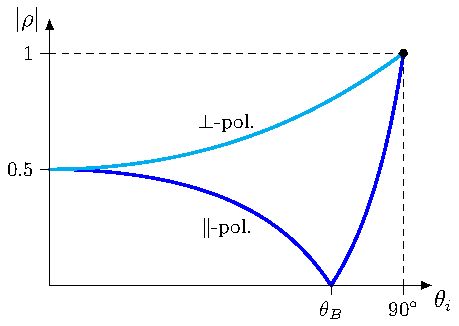
\includegraphics[width=0.5\linewidth]{img/1/Reflection-coef-function.pdf}
    \caption{Amplitude do coeficiente de reflexão em função do ângulo de incidência~\cite{silveirinha2023}}
    \label{fig:Reflection-coef-function}
\end{figure}

Retiramos as seguintes conclusões:
\begin{itemize}
    \item Para a incidência normal, as amplitudes de $\abs{\rho_{||}}$ e $\abs{\rho_{\perp}}$ são iguais.
    \item Com o aumento do ângulo de incidência, $\abs{\rho_{\perp}}$ aumenta monotonicamente, enquanto $\abs{\rho_{||}}$ diminui até ao \underline{ângulo de Brewster}, $\theta_B$.
    \item Para $\theta_i = \theta_B$, o coeficiente $\abs{\rho_{||}}$ é zero (assumindo ausência de perdas nos materiais).
    \item Para ângulos maiores que $\theta_B$, a magnitude de $\abs{\rho_{||}}$ volta a aumentar.
    \item Na incidência tangencial, onde $\theta_i \to 90^\circ$, ambos os coeficientes $\abs{\rho_{||}}$ e $\abs{\rho_{\perp}}$ tendem para um, o que indica uma reflexão total pela interface.
\end{itemize}

\begin{warning}
    É útil caracterizar $\rho_{||}$ e $\rho_{\perp}$ quando o meio 2 é um condutor elétrico perfeito. Como discutido \hyperref[warn:9]{anteriormente}, um condutor perfeito tem impedância $\eta_{PEC} = \eta_2 = 0$. Assim, para um condutor perfeito os dois coeficientes de reflexão são independentes do ângulo de incidência:
    \begin{equation}
        \rho_{\perp_{PEC}} = -1, \quad \rho_{\parallel_{PEC}} = +1.
    \end{equation}
\end{warning}

%//==============================--@--==============================//%
\renewcommand*{\thefootnote}{\fnsymbol{footnote}}
\subsubsection[Ângulo de Brewster]{Ângulo de Brewster\protect\footnotemark[2]}

Podemos obter uma expressão analítica para o ângulo de Brewster mantendo as suposições de meios sem perdas da secção anterior. Basta resolver a equação
\begin{equation}
    \rho_{\parallel} = \frac{\eta_1 \cos \theta_i - \eta_2 \cos \theta_t}{\eta_1 \cos \theta_i + \eta_2 \cos \theta_t} = 0
    \; \iff \;
    \eta_1 \cos \theta_i - \eta_2 \cos \theta_t = 0
    \; \implies \;
    \frac{1}{n_1} \cos \theta_i = \frac{1}{n_2} \cos \theta_t
\end{equation}
Através da 2\textordfeminine{} Lei de Snell, obtemos uma segunda equação que nos permitirá obter $\theta_i$ explicitamente:
\begin{equation}
    n_1 \sin \theta_i = n_2 \sin \theta_t
\end{equation}
Após uma simples manipulação algébrica pode ser visto que:
\begin{equation}
    \boxed{%
        \theta_B = \arctan\left( \frac{n_2}{n_1} \right)
    }
\end{equation}

\footnotetext[2]{%
    Uma relação geométrica curiosa é que, para $\theta_i = \theta_B$, os vetores $\mathbf{\hat{d}}^r$ e $\mathbf{\hat{u}}^i{\scriptstyle \parallel}$ são paralelos. Isto pode ser verificado observando que a condição de Brewster pode ser vista como $n_1 \sin \theta_B = n_2 \cos \theta_B$. Segundo a 2\textordfeminine{} Lei de Snell, $n_1 \sin \theta_B = n_2 \sin \theta_t$. Portanto, a condição de Brewster implica que $\cos \theta_B = \sin \theta_t$, o que só é possível se $\theta_B = 90^\circ - \theta_t$.
}
\renewcommand*{\thefootnote}{\fnsymbol{footnote}}

%//==============================--@--==============================//%
\clearpage
\begin{question}
    Considere uma onda eletromagnética plana circularmente polarizada para a direita, que se propaga no ar e incide numa camada dielétrica plana de grandes dimensões caracterizada por,
    $$
        \sigma = 0, \quad \mu_r = 1, \quad \epsilon_r = 5
    $$
    Suponha que o ângulo de incidência é de $45^\circ$ e que a densidade de potência da onda incidente junto à superfície de separação é de $10$ W/m$^2$.\\[3pt]
    a) Caracterize a onda refletida, quanto ao seu estado de polarização.\\[3pt]
    b) Determine a densidade de potência da onda refletida.

    \questionSep
    \textbf{Solução}: Vamos definir o ar como meio 1 e a camada dielétrica como meio 2. Assim,
    $$
        \text{meio 1:} \;
        \left\{
        \begin{aligned}
            \epsilon_1 &= \epsilon_0, \; \mu_1 = \mu_0 \\
            n_1 &= \sqrt{\mu_{r1} \epsilon_{r1}} = 1 \\
            \eta_1 &= \eta_0 \approx 377.0\; [\Omega]
        \end{aligned}\right.
        \qquad
        \text{meio 2:} \;
        \left\{
        \begin{aligned}
            \epsilon_2 &= 5\epsilon_0, \; \mu_2 = \mu_0 \\
            n_2 &= \sqrt{\mu_{r2} \epsilon_{r2}} = \sqrt{5} \\
            \eta_2 &= \eta_0/n_2 \approx 168.6\; [\Omega] 
        \end{aligned}\right.
    $$
    Uma vez que a onda incidente tem polarização circular para a direita, o rácio de polarização é
    $$
        p_{\text{inc}} = \frac{\underline{E}^{\text{inc}}_2}{\underline{E}^{\text{inc}}_1} = e^{-j\pi/2}
        \;\implies\;
        \underline{E}_2 = -j\underline{E}_1
    $$
    Podemos escrever a onda incidente como:
    $$
        \mathbf{\underline{E}}^{\text{inc}} = E_0 (\mathbf{\hat{u}}_{\perp} - j\mathbf{\hat{u}}_{\parallel})\, e^{-jk_0 \mathbf{\hat{d}}^i \cdot \mathbf{r}}
    $$
    Uma vez que $\mathbf{S}^{\text{inc}}_{\text{av}} = \norm{\mathbf{\underline{E}}^{\text{inc}}}^2/(2\eta_1)\, \mathbf{\hat{d}}^i$, podemos descobrir o valor de $E_0$ através da norma:
    $$
        \norm{\mathbf{S}^{\text{inc}}_{\text{av}}} = \frac{\norm{\mathbf{\underline{E}}^{\text{inc}}}^2}{2\eta_1}
        \;\iff\;
        2\eta_1\, \norm{\mathbf{S}^{\text{inc}}_{\text{av}}} = \norm{\mathbf{\underline{E}}^{\text{inc}}} = 2 E^2_0
        \;\implies\;
        E_0 = 61.4\; [\text{V/m}]
    $$
    Podemos finalmente escrever as equações dos campos refletido e transmitido:
    $$
        \begin{aligned}
            \mathbf{\underline{E}}^{\text{ref}} &= E_0 (\rho_{\perp} \mathbf{\hat{u}}_{\perp} - j\rho_{\parallel} \mathbf{\hat{u}}_{\parallel})\, e^{-jk_0 \mathbf{\hat{d}}^r \cdot \mathbf{r}} \\
            \mathbf{\underline{E}}^{\text{tx}} &= E_0 (\tau_{\perp} \mathbf{\hat{u}}_{\perp} - j\tau_{\parallel} \mathbf{\hat{u}}_{\parallel})\, e^{-j n_2 k_0 \mathbf{\hat{d}}^t \cdot \mathbf{r}}
        \end{aligned}
    $$
    Uma vez que $\theta_i = \pi/4$ e $\theta_t = \arcsin(n_1/n_2 \cdot \sin \theta_i)$, os coeficientes são dados por:
    $$
        \begin{aligned}
            \rho_{\perp} &= \frac{\eta_2 \cos \theta_i - \eta_1 \cos \theta_t}{\eta_2 \cos \theta_i + \eta_1 \cos \theta_t} = -\frac{1}{2} &\qquad \rho_{\parallel} &= \frac{\eta_1 \cos \theta_i - \eta_2 \cos \theta_t}{\eta_1 \cos \theta_i + \eta_2 \cos \theta_t} = \frac{1}{4} \\
            \tau_{\perp} &= 1 + \rho_{\perp} = \frac{1}{2} &\qquad \tau_{\parallel} &= \frac{\eta_2}{\eta_1} (1 + \rho_{\parallel}) = \frac{\sqrt{5}}{4}
        \end{aligned}
    $$
    Nestes moldes, podemos calcular a polarização das ondas refletida e transmitida:
    $$
        p_{\text{ref}} = \frac{\underline{E}^{\text{ref}}_2}{\underline{E}^{\text{ref}}_1} = \eqnmarkbox[violet]{pol-ref}{2 e^{j\pi/2}}, 
        \qquad
        p_{\text{tx}} = \frac{\underline{E}^{\text{tx}}_2}{\underline{E}^{\text{tx}}_1} = \eqnmarkbox[violet]{pol-tx}{0.89 e^{-j\pi/2}}
    $$
    \annotate[]{above, label below}{pol-ref}{pol. elíptica esq.}
    \annotate[]{above, label below}{pol-tx}{pol. elíptica dir.}

    \vspace{-1em}
    Segue o cálculo da densidade de potência de ambas:
    $$
        \norm{\mathbf{S}^{\text{ref}}_{\text{av}}} = \eqnmarkbox[violet]{Sav-ref}{\norm{\mathbf{S}^{\text{inc}}_{\text{av}}} \left(\frac{\abs{\rho_{\perp}}^2 + \abs{\rho_{\parallel}}^2}{2}\right)} = 1.56 \; \text{kW/m}^2,
        \qquad
        \norm{\mathbf{S}^{\text{tx}}_{\text{av}}} = \eqnmarkbox[violet]{Sav-tx}{\norm{\mathbf{S}^{\text{inc}}_{\text{av}}} \frac{\eta_1}{\eta_2}\left(\frac{\abs{\tau_{\perp}}^2 + \abs{\tau_{\parallel}}^2}{2}\right)} = 6.29 \; \text{kW/m}^2
    $$
    \annotatetwo{below, label above}{Sav-ref}{Sav-tx}{válido apenas quando a onda inc. tem pol. circular!}

    \footnotetext{\textbf{Nota}: \% potência refletida = $\norm{\mathbf{S}^{\text{ref}}_{\text{av}}} / \norm{\mathbf{S}^{\text{inc}}_{\text{av}}}$, mas \% potência transmitida = $(1-\norm{\mathbf{S}^{\text{ref}}_{\text{av}}} / \norm{\mathbf{S}^{\text{inc}}_{\text{av}}})$ e \textbf{não} $\norm{\mathbf{S}^{\text{tx}}_{\text{av}}} / \norm{\mathbf{S}^{\text{inc}}_{\text{av}}}$, atenção!}
\end{question}

%//==============================--@--==============================//%
\clearpage
\subsection{Reflexão Interna Total}

O ângulo incidente para o qual o ângulo de transmissão é igual a $90^\circ$ é denominado de ângulo critico e pode ser obtido através da \hyperref[subsubsec:lei-de-snell]{Lei de Snell}:
\begin{equation}
    \boxed{%
        \theta_c = \arcsin\left( \frac{n_2}{n_1} \right)
    }
\end{equation}
Quando o ângulo de incidência excede o ângulo crítico a onda sofre \textbf{reflexão interna total}, de modo que toda a energia incidente é totalmente refletida de volta para o meio de incidência.

Para $\theta_i > \theta_c$, os coeficientes de reflexão (para materiais sem perdas) têm exatamente amplitude unitária para ambas as polarizações:
\begin{equation}
\theta_i = \theta_r\qquad |\rho_{\parallel}| = |\rho_{\perp}| = 1, \quad \text{(reflexão interna total)}
\end{equation}
Este resultado pode ser depreendido para a polarização perpendicular. Admitindo $\cos\theta_t = -jC$ encontra-se que:
\begin{equation}
    \rho_{\perp} = \frac{\eta_2 \cos\theta_i + \eta_1 jC}{\eta_2 \cos\theta_i - \eta_1 jC}.
\end{equation}
Como o numerador e denominador da fração estão relacionados pela conjugação complexa, é imediato que $|\rho_{\perp}| = 1$.

Uma argumentação semelhante pode ser feita para $|\rho_{\parallel}|$.

\begin{question}
    Um tubarão nada debaixo de um barco circular de diâmetro $D$, conforme a figura apresentada. Determine o menor ângulo $2\theta_c$ dum cone imaginário dentro do qual o peixe pode nadar sem ser visto por um observador à superfície da água.
    \begin{figure}[H]
        \centering
        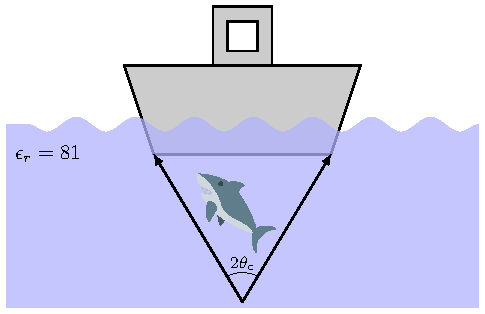
\includegraphics[width=.6\textwidth,keepaspectratio]{img/1/Shark.pdf}
    \end{figure}

    \vspace{-1em}
    \questionSep
    \textbf{Solução:} Para o peixe nadar dentro do cone sem ser visto, o ângulo dos feixes de luz que formam o cone têm de ser tais que ao incidirem entre a fronteira àgua/ar ocorre reflexão total, assim:
    $$
    \theta_\text{cone} \ge \theta_c, 
    \qquad
    \theta_c = \arcsin\left( \frac{n_\text{ar}}{n_\text{água}} \right) = 6.38^{\circ}\\
    $$
    Consequentemente,
    $$
        \boxed{\theta_\text{cone} = 6.38^{\circ}}
    $$
\end{question}


%//==============================--@--==============================//%

    % \chapter{Propagação Guiada}{example-image-duck}

    % \chapter{Radiação}{example-image-duck}

    %% bibliography
    \clearpage
    \bibliographystyle{unsrtnat} \nocite{*}
    \bibliography{refs}
\end{document}%
%//==============================--@--==============================//%